% This latex thesis example was modifed from that used in University of Michigan by Zhangping Wei (PhD student at NCCHE, OleMiss) during Feb. 2013.
% The Graduate School hasn't accept this version as the offical LaTeX thesis/dissertation template yet.
% I have tried my best to make it consistency with their requirements, but there is still NO WARRANTLY AT ALL about the correctness. Use it at your risk!
% The copyright belongs to the original author(s), you can find the original version at:
% http://aoss.engin.umich.edu/pages/current/dissertation-template.
% Have fun, folks!

\documentclass[reqno,12pt,oneside,letter]{report} % right-side equation numbering, 12 point font, print one-sided
%\documentclass[reqno,12pt,twoside,openright,letter]{report} % right-side equation numbering, 12 point font, print two-sided, Chapters start on odd pages.
\special{papersize=8.5in, 11in}	% the size of US lettler paper
\usepackage{OleMiss}         % dissertation style file modified from Rackham thesis style file
\usepackage[intlimits]{amsmath} % Puts the limits of integrals on top and bottom
\usepackage{amsxtra}     % Use various AMS packages
\usepackage{amsthm}
\usepackage{multicol}
\usepackage{amssymb}
\usepackage{amsfonts}
\usepackage{graphics}    % Add some packages for figures. Read epslatex.pdf on ctan.tug.org
\usepackage{rotating}
\usepackage{xhfill}
\usepackage[linesnumbered]{algorithm2e}
\usepackage{diagbox}
%\usepackage{color}
%\usepackage{epsfig}
%\usepackage{subfigure}  % To make subfigures. Read subfigure.pdf on ctan.tug.org
\usepackage{verbatim}
\usepackage{natbib}      % Allows you to use BibTeX
\usepackage[printonlyused]{acronym} % For the List of Abbreviations. Read acronym.pdf on ctan.tug.org
\usepackage{setspace}    % Allows you to specify the line spacing
\usepackage{hyperref}
% Z.Wei
\usepackage{comment}
%\usepackage[dvipsnames]{xcolor}
\usepackage{fancyvrb}
% redefine \VerbatimInput
\RecustomVerbatimCommand{\VerbatimInput}{VerbatimInput}%
{fontsize=\footnotesize,
 %
 frame=none,  % top and bottom rule only
 framesep=2em, % separation between frame and text
 rulecolor=\color{gray},
 %
 %label=\fbox{\color{Black}crime.txt},
 %labelposition=topline,
 %
 commandchars=\|\(\), % escape character and argument delimiters for
                      % commands within the verbatim
 commentchar=*        % comment character
}
% \usepackage[normal,labelsep=period]{caption}

\doublespacing           % \onehalfspacing for 1.5 spacing, \doublespacing for 2.0 spacing.
\newcommand{\sun}{\ensuremath{\odot}} % sun symbol is \sun
%%%%%%%%%%%%%%%%%%%%%%%%%%%%%%%%%%%%%%%%%%%%%%%%%%%%%%%%%%%%%%%%%%%%%%%%%%%%%%%
% If printing two-sided, this makes sure that any blank page at the
% end of a chapter will not have a page number.
\makeatletter
\def\cleardoublepage{\clearpage\if@twoside \ifodd\c@page\else
\hbox{}
\thispagestyle{empty}
\newpage
\if@twocolumn\hbox{}\newpage\fi\fi\fi}
\makeatother

\makeatletter
\newcommand{\rmnum}[1]{\romannumeral #1}
\newcommand{\Rmnum}[1]{\expandafter\@slowromancap\romannumeral #1@}
\makeatother
%%%%%%%%%%%%%%%%%%%%%%%%%%%%%%%%%%%%%%%%%%%%%%%%%%%%%%%%%%%%%%%%%%%%%%%%%%%%%%%

\begin{document}

\setlength{\parindent}{0.5in}
\bibliographystyle{Bibfiles/agu04}    % Set the bibliography style: agu04.

% Title page
\titlepage{SENTIMENT OF THE UNION\break \textit{Analyzing Tone in Presidential State of the Union Addresses}}
{by \\
Chase Rydeen}
{Oxford \\
May 2018}	% The graduation Date
{Dr. Dawn Wilkins} % First Reader
{Dr. Naeemul Hassan} % Second Reader
{Dr. Yixin Chen} % Third Reader

% Begin the front matter as required.
\initializefrontsections

% Optional Frontispiece
%\frontispiece{\includegraphics[width=6in]{Intro/Happy} Find a cool picture to go here.}

% Optional, but recommended, Copyright page
\copyrightpage{Copyright}{Chase Rydeen}

% Page numbering. If you don't include a frontispiece or copyright page, you'll need to change this for two-sided printing.
\makeatletter
\if@twoside \setcounter{page}{4} \else \setcounter{page}{1} \fi
\makeatother

% Optional in-dissertation Abstract Page
\startabstractpage
As the machine learning and data science craze sweeps the nation, the implications and implementations are vast.
This paper takes a look at both of them through the lens of a topic of national importance, at the very least for the United States.
This topic is the words used by past Presidents of the United States, which are being pulled from their State of the Union Addresses.
These two broad subjects are implemented in varying degree by means of Natural Language Processing (NLP), of which this paper is centered around.
Natural Language Processing pulls heavily from both of these two categories to enable effective analysis of text-based data.
Using NLP, a sentiment analysis was conducted on the Addresses to gain further insight into the tone used by Presidents over the course of history.
This paper shares the methodology used to conduct this sentiment analysis and discusses how it was presented and \href{https://turing.cs.olemiss.edu/~dcrydeen/thesis/index.html}{visualized}.
\label{Abstract}

% Optional Dedication page
\startdedicationspage
To be completed.
\label{Dedication}

% Optional Acknowledgements page
\startacknowledgementspage
Thank you so much to Dr. Wilkins for guiding me on this long journey and always being there when I need her. You are a true inspiration and have been so influential in my undergraduate career, and I'm so thankful for all your advice and help with this paper and this thesis.

Thank you Dr. Hassan for teaching me all I know about information visualization and D3.js to make the visuals for this thesis.


\label{Acknowledgements}

% Optional Preface page
%\startprefacepage
%\input{Preface}
%\label{Preface}

% Table of contents, list of figures, etc.
\tableofcontents     % Required
\listoffigures       % Required if there is more than one figure
\listoftables        % Required if there is more than one table
%\listofmaps          % Required if there is more than one map
%\listofappendices    % Required if there is more than one appendix
%\listofabbreviations % Optional. Abbreviations should be stored in a file named abbr.tex

\startthechapters
% The individual files for each of the chapters are put here.
% Save each chapter of your thesis to a seperate tex file
% and then use the \input command to include this file in your
% thesis.  For instance you can save a file to "intro.tex" and
% then type \input{intro}.

 \chapter{INTRODUCTION}
 \label{chap:Introduction}
 \input{Chapter1/Chapter1}

 \chapter{CORPUS}
 \label{chap:Corpus}
 \section{State of the Union Addresses}
The main textual data that was collected to be processed was all of the Presidential State of the Union addresses, from George Washington's first address to Barack Obama's last address.
The text source was initially pulled from a Presidential Address Repository [\cite{presrepo}].
The text came in a large text file that contained every speech and it was split in to individual text files for each individual address to allow for easier processing.
The addresses vary widely in length and content, which is also of significant note when analyzing and comparing these addresses across the timespan of the existence of the United States.
George Washington's first address was just over a thousand words and seventeen paragraphs, whereas Barack Obama's final address was just over 5,400 words and was 78 paragraphs long.

\subsection{Change in Purpose of State of the Union Address}
The length is the most notable change in the State of the Union Addresses over time, but there are important factors to consider as well that could potentially impact how the addresses are given from year to year.
When the Presidential Addresses first started with George Washington, it was not intended to be a recurring event [\cite{teten2003evolution}], but it soon began to grow to a tradition so that the president could publicly address the people and inform them of the current events of the country.
Over the years, the Presidential Address has taken on many forms, in spoken word, in written letter, in radio broadcast, and, nowadays, on live television broadcast.
The Presidential Address shifted from the yearly Presidential update, sometimes the only time people would hear directly from the President, to a formalized briefing to inform the public in an organized manner of the current state of affairs and push forward a President's agenda for the upcoming term [\cite{teten2003evolution}].
While that has always been a goal of the addresses, it has become more of the central focus over the course of time, due to technological innovations and changes in media coverage.
Nowadays, citizens of the United States can read in real-time about the decisions of the Presidency and the Presidents political moves without needing to listen to an annual speech to become updated on their agenda and goals for the year to come.
It is a subtle, yet interesting shift in how the addresses are approached, but even these purposes could change, depending on the person giving these orations, an important factor to consider also.

\subsection{Presidential Personality}
Another important factor in how the Presidential State of the Union Addresses are given is the personality of the President that is giving them.
This is a rather intangible element of the speeches that can be hard to quantify but is very important to note.
Most people have a certain disposition towards being more optimistic or pessimistic, and that can become apparent in the speeches given.
The important topic being considered here is tone, which can be heavily influenced if the President giving the speech tends to be more realistic or optimistic in their outlook on the world.
Some President's may see the State of the Union as a chance to rally the nation and project positivity and support for their platform for years to come, whereas others might see it as a good opportunity to have a nation-wide reality check and bring the citizens in-line with what needs to be done for the good of the nation [\cite{teten2003evolution}].

\section{Statistical Summary}
It is important to have an understanding of the speech data itself before diving in to this research, since otherwise it won't be as meaningful and it will be harder to draw conclusions.
The full statistical summary for the data can be found in Table \ref{stat:one}.
This can be explored to search for trends in the data and familiarize oneself with an overall perspective on the data.
Some information of note: 
There are a total of 230 Presidential Addresses given by 42 Presidents, making the average number of addresses per president 5. 
There are 26 Republicans and 16 Democrats, which makes their percentages 62\% and 38\%, respectively.
The first three columns are self-explanatory and the latter two are described below.

\subsection{Lexical Diversity}
Lexical diversity is a metric that is used to represent the amount of unique words in any given passage of text and thus the overall complexity of the text [\cite{johansson2009lexical}].
Lexical diversity is calculated by dividing the number of unique words in a text by the total length of the text.
The resulting number is between 0 and 1 and the closer to 1, the more diverse the lexicon, so a value close to 1 can be interpreted as being more complicated to read.
The patterns here can be confounding by sheer length of a text but it remains an important metric to see how complex a particular selection of text is.
The nature of this calculation makes it more interesting when comparing two pieces of text that are similar in length to see the lexical diversity between the two.
This calculation was performed for each State of the Union address and then all of the scores for each President were averaged together to get an average lexical diversity for each President.

\subsection{Grade Level}
Calculating grade level is a slightly more involved process that involves an algorithm that computes grade level based on two factors: average sentence length and average syllables per word.
This formula was created in 1975 to determine the readability of documents for Navy enlisted personnel [\cite{kincaid1975derivation}]
The first factor is relatively easy to calculate, but the second is slightly more tricky as syllables can be a lot more difficult to distinguish in plain text processing fashion.
Luckily, there is a Python plugin called textstat with a built-in Flesch-Kincaid function that has a corpus of syllabled words and it was used to calculate grade level.
You can see how the formula is used in Equation \ref{eq1}.

\begin{equation} \label{eq1}
    0.39\ (\frac{total\ words}{total\ sentences}) + 11.8\ (\frac{total\ syllables}{total\ words}) - 15.59
\end{equation}

\begin{singlespace}
\begin{table}[tp]
\begin{center}
 \begin{tabular}{||c | c c c c||}
 \hline
 President & \# of Addrs. & Avg \# Words & Lex Diversity & Grade Level \\
 \hline\hline
 George Washington & 8 & 2096.0 & 0.3762 & 18.55 \\ 
 \hline
 John Adams & 4 & 1801.0 & 0.369 & 17.925 \\
 \hline
 Thomas Jefferson & 8 & 2605.0 & 0.3376 & 18.0 \\
 \hline
 James Madison & 8 & 2729.0 & 0.3433 & 20.825 \\
 \hline
  James Monroe & 8 & 5326.0 & 0.2493 & 16.462 \\
 \hline
  John Quincy Adams & 4 & 7864.0 & 0.2327 & 19.25 \\
 \hline
  Andrew Jackson & 8 & 10708.0 & 0.2042 & 19.2 \\
 \hline
  Martin van Buren & 4 & 11411.0 & 0.2036 & 20.15 \\
 \hline
  John Tyler & 4 & 8560.0 & 0.2291 & 18.475 \\
 \hline
  James Polk & 4 & 18173.0 & 0.1525 & 17.275 \\
 \hline
  Zachary Taylor & 1 & 7678.0 & 0.2346 & 17.2 \\
 \hline
  Millard Fillmore & 3 & 10612.0 & 0.2224 & 16.967 \\
 \hline
  Franklin Pierce & 4 & 10545.0 & 0.2192 & 19.15 \\
 \hline
  James Buchanan & 4 & 14247.0 & 0.1797 & 15.05 \\
 \hline
  Abraham Lincoln & 4 & 6999.0 & 0.2639 & 13.675 \\
 \hline
  Andrew Johnson & 4 & 9690.0 & 0.2294 & 15.9 \\
 \hline
  Ulysses S. Grant & 8 & 8232.0 & 0.2391 & 15.938 \\
 \hline
  Rutherford B. Hayes & 4 & 8692.0 & 0.2363 & 16.325 \\
 \hline
  Chester A. Arthur & 4 & 5045.0 & 0.3252 & 13.6 \\
 \hline
  Grover Cleveland & 4 & 12478.0 & 0.2236 & 17.45 \\
 \hline
  Benjamin Harrison & 4 & 13881.0 & 0.1976 & 14.7 \\
 \hline
  Grover Cleveland & 4 & 14969.0 & 0.2121 & 16.35 \\
 \hline
  William McKinley & 4 & 16901.0 & 0.1977 & 15.8 \\
 \hline
  Theodore Roosevelt & 8 & 19793.0 & 0.1732 & 14.975 \\
 \hline
  William H. Taft & 4 & 17594.0 & 0.1868 & 17.025 \\
 \hline
  Woodrow Wilson & 8 & 4384.0 & 0.2768 & 15.05 \\
 \hline
  Warren Harding & 2 & 5738.0 & 0.2768 & 13.5 \\
 \hline
  Calvin Coolidge & 6 & 8707.0 & 0.2306 & 11.783 \\
 \hline
  Herbert Hoover & 4 & 6489.0 & 0.2566 & 14.15 \\
 \hline
  Franklin D. Roosevelt & 12 & 3991.0 & 0.3002 & 12.0 \\
 \hline
  Harry S. Truman & 8 & 8405.0 & 0.2321 & 10.475 \\
 \hline
  Dwight D. Eisenhower & 9 & 6103.0 & 0.2751 & 12.3 \\
 \hline
  John F. Kennedy & 3 & 5816.0 & 0.289 & 12.233 \\
 \hline
  Lyndon B. Johnson & 6 & 4917.0 & 0.2707 & 10.017 \\
 \hline
  Richard Nixon & 5 & 4002.0 & 0.2692 & 11.78 \\
 \hline
  Gerald R. Ford & 3 & 4649.0 & 0.2865 & 10.767 \\
 \hline
  Jimmy Carter & 4 & 11410.0 & 0.2427 & 11.05 \\
 \hline
  Ronald Reagan & 7 & 4731.0 & 0.2963 & 9.557 \\
 \hline
  George H.W. Bush & 4 & 4396.0 & 0.285 & 7.8 \\
 \hline
  Bill Clinton & 8 & 7528.0 & 0.2207 & 9.35 \\
 \hline
  George W. Bush & 9 & 4888.0 & 0.2883 & 9.122 \\
 \hline
 Barack Obama & 8 & 6738.0 & 0.2465 & 8.412 \\
 \hline
  Donald Trump & 1 & 5199.0 & 0.3043 & 8.4 \\
 \hline
\end{tabular}
\end{center}
\caption{Presidential Summary Statistics}
\label{stat:one}
\end{table}
\end{singlespace}

\section{Information Visualization}
An important part of this research is also concerned with how best to display the resulting information in an effective and easy-to-understand manner.
There is an entire field dedicated to how to best display technical information and data and how to convey it to large groups of people with little technical background [\cite{fekete2008value}].
This is important with data such as the sentiment score being processed here, as the long numbered sentiment scores are intimidating and without any context, data is meaningless.
The context here is contained within the graph used to display the sentiment score data and interactive features were implemented to help users engage with the data in a more meaningful fashion.
The data in this research is quantitative and since the Presidential Addresses are given in chronological order, time was used on the x-axis and the data lended itself nicely to a Scatter Plot.
This scatter plot will be discussed more in-depth in the following section.


\subsection{Word Cloud}
A word cloud is a collage of words that displays word frequencies for a certain set of text data, with the relative size of each word being determined by the frequency with which that term is used in the text [\cite{heimerl2014word}].
An example can be seen in Figure \ref{fig:wordcloud1} that shows the word cloud for all of Jimmy Carter's words he used for every one of his State of the Union addresses.
A second example can be seen in Figure \ref{fig:wordcloud2} where a term is selected and the word cloud dataset is restricted to the contents of that particular presidential address.
Word Clouds are an interesting visual since they provide quick reference to see what a President's most used terms are, as well as being another interesting way to engage the data in a slightly different context.
Word Clouds themselves are often criticized since it is a poor way to visualize data and it is hard to objectively compare two words in a word cloud because the frequency values are encoded using area, which is a very difficult encoding for humans to interpret [\cite{cui2010context}].
In this case, the word cloud is used merely to complement the line plot visualization that will be introduced next chapter that provides insight into the main purpose of the research, and the word cloud provides a different way of visualizing the data source itself.

\begin{figure}
  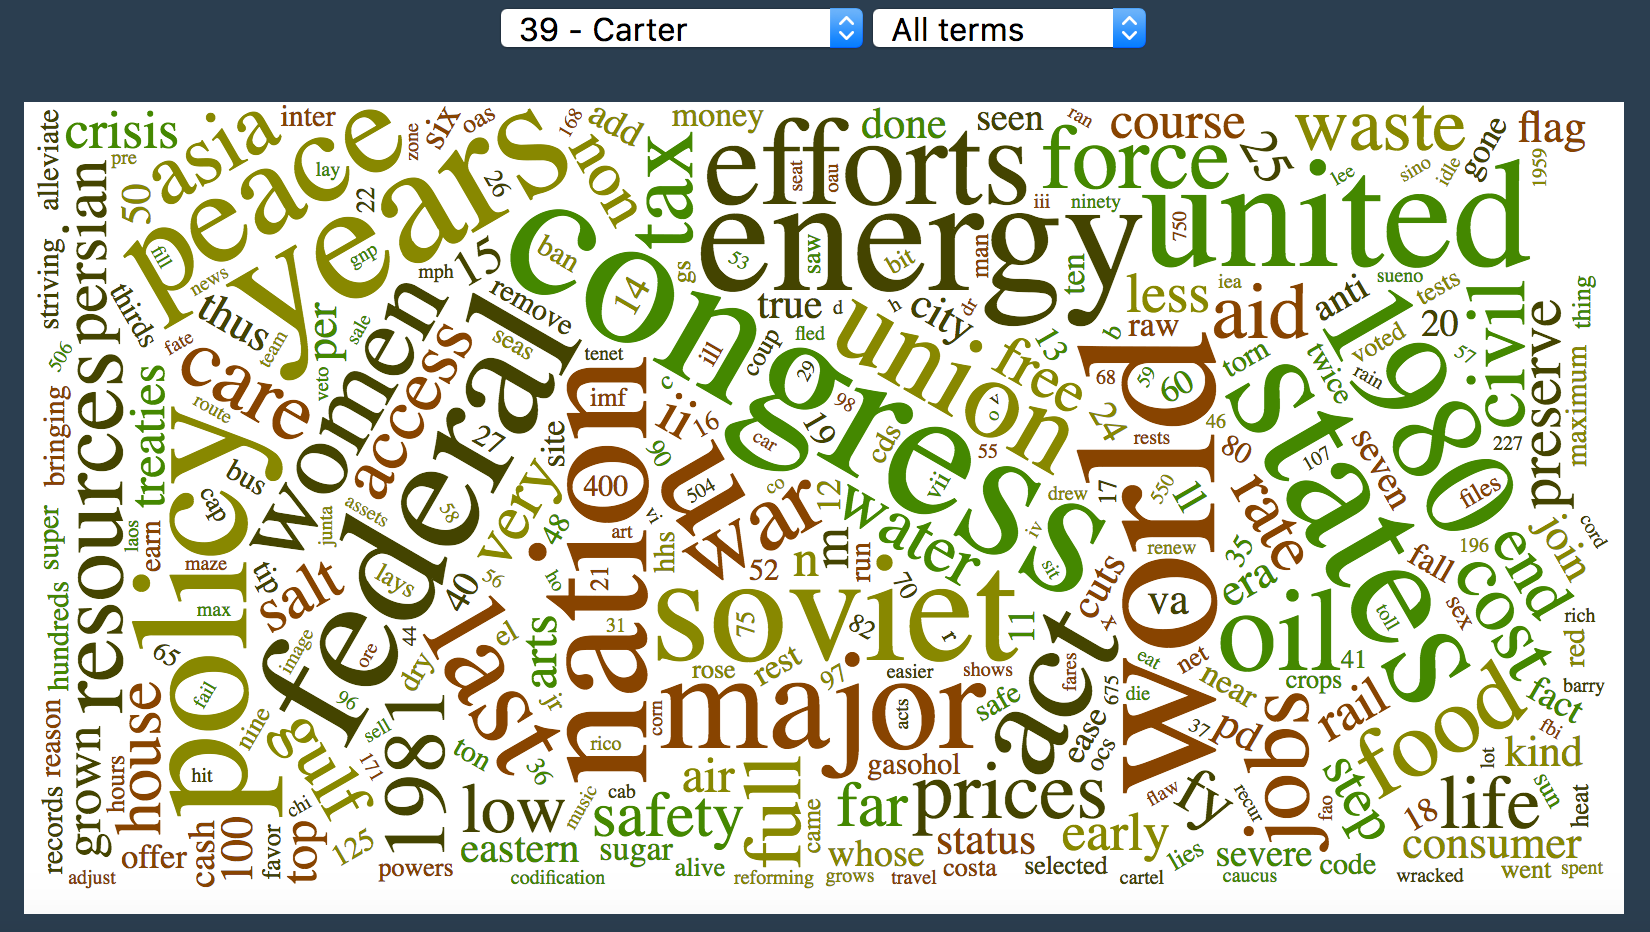
\includegraphics[width=\columnwidth]{images/Wordcloud.png}
  \caption{Example Word Cloud showing all terms for Jimmy Carter}
  \label{fig:wordcloud1}
\end{figure}

\begin{figure}
  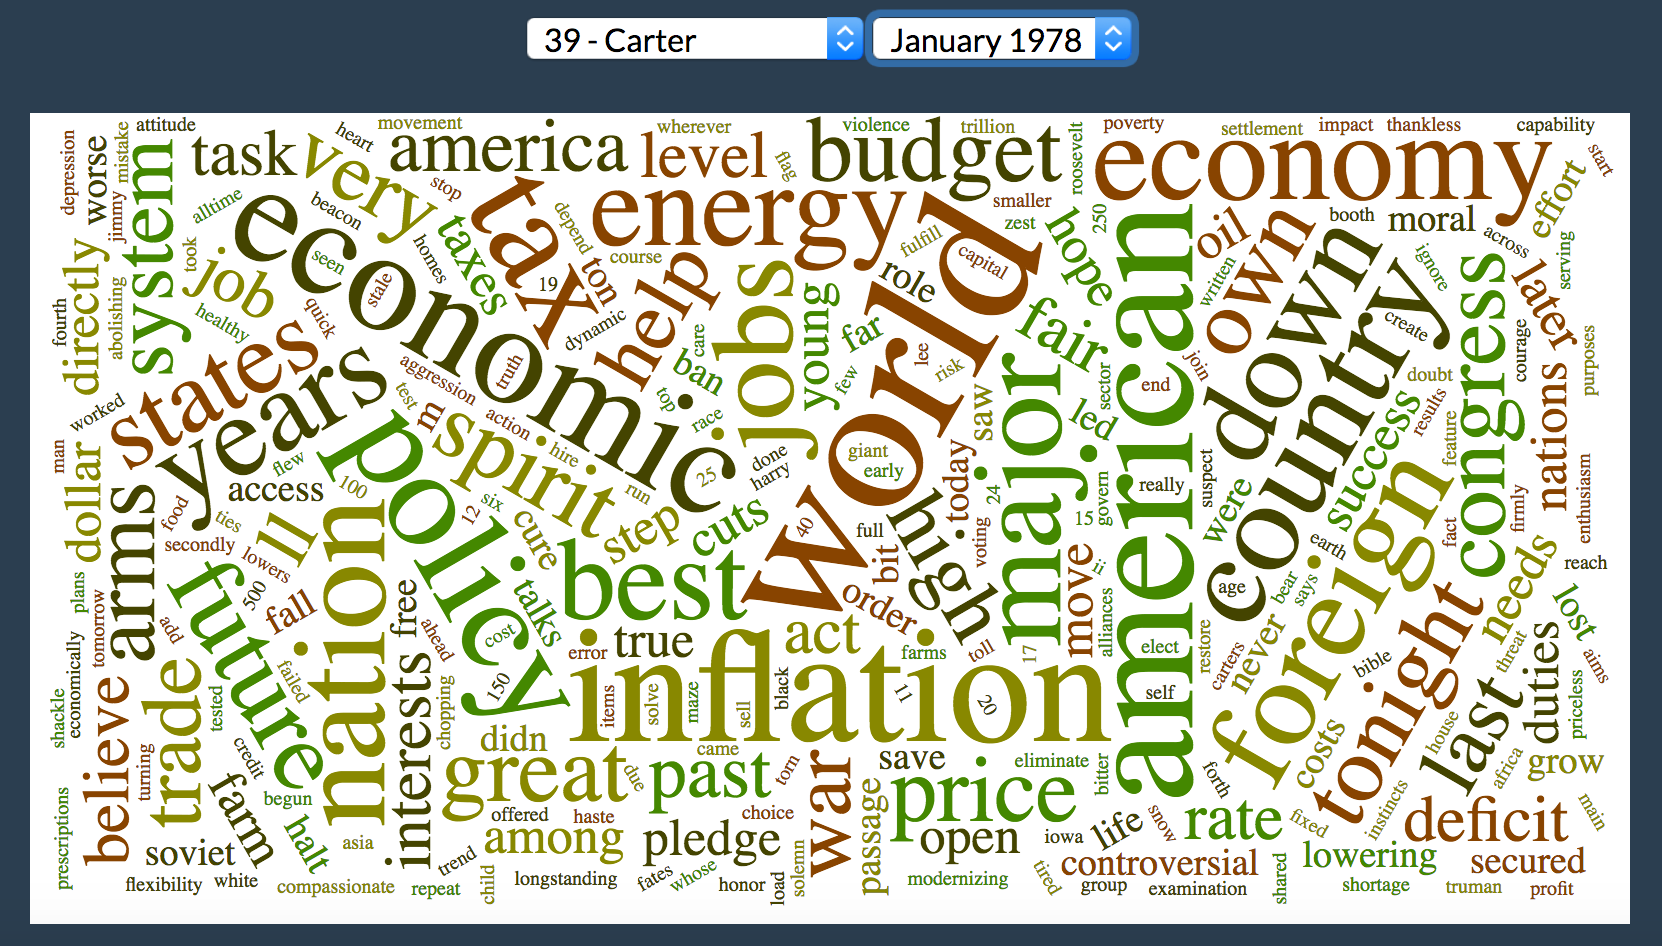
\includegraphics[width=\columnwidth]{images/Wordcloudterm.png}
  \caption{Example Word Cloud showing 1978 term for Jimmy Carter}
  \label{fig:wordcloud2}
\end{figure}

\subsection{D3}
D3.js (D3) is the JavaScript Library used to create the visualization mentioned in the previous section and another mentioned in a future section.
D3 uses pre-built JavaScript functions to select, elements, create SVG elements, style them, or add dynamic effects or tooltips to them [\cite{bostock2011d3}].
D3 also has a handy library that creates word clouds that was used in this research, it takes in an input array in JSON format with the words and their frequencies in decreasing order and draws the words with their relative sizes on the HTML canvas.
There is a bit of a delay on the drawing of the word clouds, since instead of saved images of the word clouds, the program is actually drawing all of them in realtime and just swapping out the JSON data source depending on which President is selected in the dropdown menu at the top of the page.

\section{Results}
The bulk of this information is used later for processing, but it is important to understand the data source as well, before diving in to predictions using it.
The importance and purpose of the State of the Union address is important here since it has a heavy-handed influence on the content and message behind the Presidential Addresses.
It is important to note that the party breakdown, with 26 Republicans and 16 Democrats, makes their percentages 62\% and 38\%, respectively.
These numbers aren't exactly correct, as the lesser-known and ephemeral early parties were placed in to either Democrat or Republican based on their policy positions.
For example, Democratic-Republicans were assigned Republican as that party eventually became the common day Republican party, and the Whig Party was assigned to Republican as well as it was created from former of the Democratic-Republican Party.
This was done in order to maximize the effectiveness of the prediction algorithm that will be discussed later on.
The statistics here are important as they provide more insight into the data being processed and provide a more concise view into what is being handled.
Table \ref{stat:one} has some intriguing patterns and trends to analyze and show.

\subsection{Average Address Length}
The average length of the Presidential Address has changed drastically over time, as its purpose and importance fluctuated.
George Washington, when he gave his first address, didn't think that it would be a reoccurring event, but thought it necessary to inform the citizens of the current state of affairs of the country, and this precedent was followed for much of the early history of the United States [\cite{freeman1948george}].
The relatively short length of the early Presidential Addresses shows this, as it was short and brief.
It was meant to inform the people of what is happening in the country and was used primarily to disperse information to the citizens.
This slowly began to change over the years and the change can be seen in just the average number of words in the addresses.
This change indicates the increasing importance of the State of the Union address as a chance to communicate with the citizens at large and use that attention to push an agenda and connect with the voters.
The State of the Union address became a much larger deal as President's used it to communicate with the entirety of the nation to ensure them of the success of the nation and its status, peaking with Theodore Roosevelt averaging almost 20,000 words per Presidential Address.
Shortly after, however, the length of the addresses had a tremendous drop-off from Taft at 17,000 words to Woodrow Wilson at 4,300 words, which can likely be attributed to the emergence of World War I.
The country was involved in a major war effort and the fanfare and policy pushing of State of the Unions past were cleared out of the way for the focused messages of State of the Union addresses to come.
These were defining times in the world, and with a major conflict to unite all people in the country, the State of the Union addresses became more condensed and focused on the important aspects at hand.
These shorter addresses were used to encourage the country and assure them of the success of the war effort and keep country-wide morale high and trying not to distract them for too long.
From this major change and in to the modern era, the State of the Union address has stabilized around 5,000 to 10,000 words, keeping to an average length and the TV equivalent of roughly an hour to an hour and a half, long enough to keep people's attentions and effectively convey a president's reflections on the past year and goals for the next.

\subsection{Lexical Diversity}
Lexical Diversity, which was introduced previously, is also interesting to note here and it generally follows the same pattern as average length, just in the reverse fashion.
As one would expect, the more words that are spoken, the less overall unique words are going to be spoken.
This is most evident when examining the lexical diversity of George Washington and that of Teddy Roosevelt.
George Washington had notoriously short State of the Union Addresses so his average lexical diversity was 0.3762, whereas Teddy Roosevelt has an average lexical diversity of 0.1732, which makes sense since his average length is almost ten times greater than that of George Washington's.
This provides more important insight in addresses that are similar length to one another and provides a deeper insight into the speech-writing process and how word selection is important when communicating information to large swathes of people and needing to be considerate of their education levels.

\subsection{Grade Level}
Another metric that complements Lexical Diversity that needs to be considered is Grade Level, which was mentioned previously and it is computed using the Flesch Kincaid mentioned above.
The scores seen here may seem rather high but it is understandable given the change in how Americans speak over time.
Speakers in Early America were known to have a rather complicated way of talking and in order to make it to the office of President one had to be sufficiently educated to get elected by the public.
This pattern shows in the high grade level throughout the early and mid history of the United States as most of the early presidents were college-educated, a rarity of the time, and had a more sophisticated vocabulary than the common man.
Also the early speeches were often given in front of Congress and with no means of distributing the speech widely, the intended audience was mainly Congress, so the early Presidents did not really have a need to simplify their language to communicate effectively to the common man as was done by the newspapers that talked about the Address [\cite{ziff1991writing}].
The grade level gradually has decreased over time, which has as much to do with the greater reaches the address has, as it does with the way modern day media collects sound bites of presidential addresses.
In the modern era, when a President gives a speech, only a small amount of the actual speech is rebroadcast when the media is discussing it, so the ``sound bite" phenomenon has arisen in State of the Union addresses, which has had a transitive effect on the Flesch-Kincaid grade level calculation.
The media only takes small snippets of what the President says to convey major policy positions, which has had the effect that most statements are kept short in order to summarize points and clearly convey what positions the President has in as short a form as possible [\cite{paletz1977presidents}].
And since one of the calculations for the grade level calculation is average words per sentence, this brings down the grade level of the speech as the President attempts to become more clear in their purpose and position to effectively convey their thoughts and feelings in a short sound bite that could be taken from their speech.

 % Sentiment / Preprocessing /SOTU Addresses
 \chapter{SENTIMENT ANALYSIS}
  \label{chap:Sentiment Analysis}
  \input{Chapter3/Chapter3}

 \chapter{MACHINE LEARNING}
 \label{chap:Machine Learning}
 Machine Learning has emerged as booming field in Computer Science that provides a lot of opportunities for innovation and growth.
The important thing to know about machine learning is what is in the name: teaching machines to learn.
Through various approaches and algorithms it is possible to feed these machines input data and coach them to predict outcome events without being explicitly programmed to do so [\cite{hansen1990neural}].
Machine Learning algorithms come with a caveat though that unfortunately this research exhibits, and that is that effective machine learning is difficult because finding patterns is hard and often there isn't enough training data available to effectively train the algorithm to make predictions.
The data here is large but rather minute compared to the large amounts of data normally used to train such learning algorithms.
As such, the results achieved here aren't as strong as one would hope but this research establishes an approach that could be expanded and fed more data to achieve a more effective result.

Machine Learning can refer to many different topics as it is a broad field, but in this research the learning algorithms used were Neural Network, Naive Bayes Classifer, and Decision Tree.
All of these fall into the supervised learning category of machine learning wherein a training set of data is input, along with the target outcome that allows the models to use this data and output target to learn how to predict the outcome [\cite{dietterich1998approximate}].
Before the learning algorithms are discussed more in-depth it is important to understand the data that was produced to create the learning set and how it was used.

\section{Topic Classifier Sets}
An important part of the latter half of the preprocessing work for this research was the topic classifier sets.
At first, the sentiment score was calculated for each presidential address with an overall score from -1 to 1, indicating their tone when delivering that address.
After these were calculated, they were analyzed to look for trends in each president's tone to see if there were any interesting patterns.
As an additional breakdown to see if there was any more context-specific information that could help determine a president's political party, topic categories were added to diversify the scores of the presidents.

Four Presidential Addresses were chosen (Washington, Lincoln, Kennedy, Obama) and manually read to discover what words were being used when talking about certain general topics within the United States.
The twelve topics that were identified were: crime, economy, education, energy, environment, family, foreign affairs, government, job, religion, terrorism, and war.
Text files were created using the trigger words that were collected for each major topic.
The trigger words were pulled from the four addresses mentioned above and from various other addresses as they were skimmed through.
During the algorithm, these text files are converted into arrays and as a sentence is being processed, it is scanned for these trigger words and if it has one of those words then it assigned to that topic.
Then the sentiment analysis is conducted on each of the sentences within each of the categories to obtain a topic sentiment score for each President.
The implementation of this part of the algorithm can be seen in Algorithm \ref{alg:classification} on the next page, and the trigger words are used starting on line \ref{alg:classification:topic}.

This processing was conducted on every address and the sentiment score for each topic was found for each President, which resulted in a vector for each address that had their overall sentiment score and the sentiment score for each topic covered in the address.
These scores for each address were then averaged together to create an overall vector for each president that could be used for classification and learning to learn their political party.
This vector consisted of 15 values (the President's name, the overall sentiment score, 12 of the topic sentiment scores mentioned above, and the President's political party) to be used for learning.
For example, George Bush's vector was ['Bush', 0.1340853948691, 0.1302164475371004, 0.13079766376531318, 0.13296404930509467, 0.13296404930509467, 0.13743239837292998, 0.13949090904366207, 0.14036831555702362, 0.1434021113795079, 0.14341784426710505, 0.14306495549111073, 0.14278963481416337, 0.14030583896785492, 'Republican'].

\begin{singlespace}
\begin{algorithm}[H]
\DontPrintSemicolon
\KwIn{All State of the Union Addresses}
\KwOut{The sentiment score for each Presidential Address for each category.}
\BlankLine
open all .txt files and store them in lists of special category trigger words\;
\For{each address in the State of the Union Addresses}
	{format address\;
	split address in to sentences\;
	\For{each sentence in the address}
		{add sentence to 'overall' category\;
		\If{sentence contains category trigger word \label{alg:classification:topic}} 
		{add sentence to category}
	\For{each category}
		{append list of sentences for that category to an overall list}
	\For{each topic in the overall list}
		{\For{each word in the topic}
			{create word count for each word and store it in a dictionary\;
			\If{previous word negator}
				{increment negator counter for that word by one}
			\If{previous word intensifier}
				{increment intensifier counter for that word by one}
			}
		\For{each word in the dictionary}
		{\If{word is in lexicon}
		{\If{length of negators[word] != 0}
		{Subtract length from total count for that word}
		}
		\If{length of intensifiers[word] != 0}
		{Raise length number of scores to the power of 2}
		Calculate the Sentiment Score by multiplying the number of occurrences of the term by the score in the lexicon.
		}
		}
	}
	}
	
\caption{Sentiment Analysis Algorithm}
\label{alg:classification}
\end{algorithm}
\end{singlespace}

\section{Normalization}
As an added measure to clearly show the differences between different vectors, each of the values was normalized from -1 to 1 using a simple normalization algorithm.
This normalization process aided in distinguishing the minute differences that manifest themselves when the data is more spread out on a greater range.
The normalization method can be seen in Algorithm \ref{alg:two}.

\begin{singlespace}
\begin{algorithm}[H]
\DontPrintSemicolon
\KwIn{Master array (an array of all the Presidential vectors)}
\KwOut{The Master array (Now with all values normalized)}
\BlankLine
\For{array in master}
	{old\ min = min(array)\;
	old\ range = max(array) - old\ min\;
    	new\ min = -1\;
   	new\ range = 2\;
    	array \= [float((n - old\_min) / old\ range * new\ range + new\ min) for n in array]\;
	new\_\ master.append(array)}
\caption{Normalization Algorithm}
\label{alg:two}
\end{algorithm}
\end{singlespace}

\section{Neural Networks}
Neural Networks take their name because they are trying to mimic and that is of a human's brain and its biological neural networks that allow it to make decisions [\cite{hansen1990neural}].
This concept was mirrored and used to produce neural networks that are fed input data that is labeled as either exhibiting a behavior or not exhibiting a behavior and using that data to predict the unknown label of future inputs.
The neural network has no inherent knowledge about the sentiment scores inserted into them, nor the political party label but it merely uses this data to learn patterns and uses these patterns to predict the political party of an unknown president using their sentiment scores.
This first step of learning from data that is labeled is called the training phase.
The training phase is important since the effectiveness of the algorithm relies entirely on the algorithm being trained correctly and effectively [\cite{hepner1990artificial}].
The goal is to have a diverse set of inputs to give the algorithm a range of data, and then tell it how many times to repeat over the data to learn it.
Finding the sweet spot of how many repetitions to utilize when having the algorithm learn the input data is very important, as too many repetitions causes the algorithm to confine itself to just the input data and it will lose the ability to generalize patterns to predict outcomes correctly, and too few repetitions prevents the algorithm from interacting with the data enough to draw meaningful patterns and conclusions from it.

A visualization for how a neural network works can be seen in Figure \ref{fig:nndiagram} [\cite{juan2013nndiagram}].


\begin{figure}
\begin{center}
  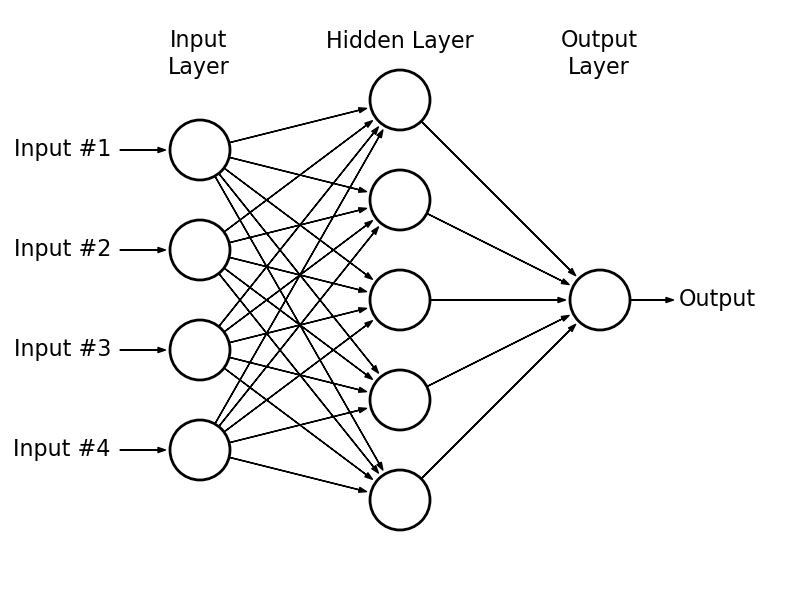
\includegraphics[width=250pt]{images/nndiagram.png}
  \caption{Neural Network Diagram}
  \label{fig:nndiagram}
  \end{center}
\end{figure}



\section{Naive Bayes Classifier}
A Naive Bayes classifier functions in a very similar fashion to that of a neural network but it is less of a black box approach and more of a statistical approach.
Using the input and target data, the Naive Bayes classifier uses a statistical model to predict values rather than strictly pattern recognition [\cite{murphy2006naive}].
Naive Bayes has actually been discovered to handle small amounts of data better than neural networks so it was important to add here since both have their strong suits in predicting values.
Naive Bayes is a much simpler algorithm which can limit its performance and effectiveness as it attempts to fit its training data too closely, causing it to lose accuracy, whereas a neural network's complexity can actually overfit the data, which makes it weaker at predicting data outside the input data set.

\section{Decision Tree Classifier}
A Decision Tree Classifier functions in almost the exact same way that Naive Bayes does, but instead of predicting one output value, a decision tree examines the data to find steps it could take to make the correct prediction.
Using these steps, a Decision Tree produces a list of steps it iterates through for each value and uses the outcome of each of the steps to predict the output value.
This is effective with data that shows more trends and is sufficiently spread out, but this function struggled with this data as the decisions it made weren't clear and it overfit itself to the data which caused performance issues in this research [\cite{dietterich1995overfitting}].
A Decision Tree can be useful since it produces a model in a human readable fashion that gives insight into how it makes a prediction, which can allow for easier fine-tuning of the data and the algorithm to produce the best results.
Much of machine learning can be a black box approach and this insight in to the inner workings of this algorithm simplifies it, but also limits it as this simplicity makes the algorithm not always as effective in its predictions.

\section{Leave-one-out Cross-validation}
In order to evaluate the effectiveness of the algorithm, leave-one-out cross-validation was used.
This validation method works by iterating over the data and hiding one of the points of data and uses the remaining data points to predict the hidden one [\cite{tzutsung2015validation}].
This is then repeated for each of the data points to be the hidden one.
In this research, each address is represented as a vector of 13 numbers and two strings, indicating the sentiment scores for each category as well as the overall score and the final value is the political party the president belongs to.
Then, using these vectors, one of them is hidden, and the rest of the vectors are used to predict the values for the hidden vector.
This process is then repeated for each of the vectors until all of them have been the hidden one and had their output predicted.
This validation method ensures the algorithm is working properly and can properly predict a set of values using the existing data set.

\section{Results}
The results from the machine learning algorithms were less than stellar but provide interesting insight into the problems at hand regardless of this.
The breakdown of Democrat and Republican is 38\% and 62\% respectively.
So, ideally the desired accuracy for an effective learning algorithm would be reasonably above 62\% as you could successfully get 62\% every time by predicting Republican for every single president.
Unfortunately, the results achieved for these machine learning algorithms were 59.5\% for the Neural Network and 35.71\% for the Naive Bayes Classifier and Decision Tree.
These accuracy numbers are less than satisfactory but there is much to say about the data being handled and how effective translating qualitative into quantitative data works.
Text data at its heart is qualitative data since there is feeling and tone and intangible elements of speech that one can't quite quantify just yet but there is a way to do it.
This research ran into many of these same roadblocks that come with translating text data into numeric data as some of this intangible meaning is lost and has to be reproduced mechanically to reach necessary conclusions about the data.

These results are less than astounding but it is interesting how much better the neural network performed than the statistical measure of the Naive Bayes.
So the patterns drawn from the neural network were stronger indicators of party alliance and even though the data source was small, the neural network performed stronger even though typically the opposite is the case when comparing these two approaches as was mentioned previously.
The Decision Tree Classifier has the same accuracy as the Naive Bayes as they both function similarly when the data set is small and they function very similarly in this research.
Instead of creating a pattern to discern the vector values for each presidential party, the decision tree shows that it assigned the sentiment scores value to that category and if the values matched another one, it would look at the party of the matched one and assign it that, all the way down the list of categories.
This overfitting caused the algorithm to focus too much on early results and not look at the whole data set before predicting a value which caused it to have an interestingly low prediction accuracy rate, worse than picking every party the same [\cite{dietterich1995overfitting}].
The concept and algorithms themselves are interesting but the accuracy and results are less than convincing about whether this can adequately be proven as a relation.

\subsection{Vector Analysis}
To add more context to the vector creation, here are two vectors from the calculations that will be interpreted.
The two vectors can be seen in Table \ref{table:vector} below, and a full list of all of the vectors can found in the appendix [Here - To be completed].

The two excerpts are a small portion of the data collected but they both show interesting trends in tone across the different topics.
Also, to be noted is the fact this these numbers are an average for all of the addresses given by the President and not single term.
This is especially pertinent since George Bush had an extremely low sentiment score on his address immediately after 9/11 but his other ones were generally higher and averaged him out to a more positive sentiment score.
Overall and across the categories, Abraham Lincoln has lower sentiment scores than Bush and actually his overall sentiment score is fairly higher than any one of his topic scores.
This indicates a topic not featured here that he had an overwhelmingly positive tone on that averaged his overall score higher, or just a general positive mood not directed towards any specific topic.

Abraham Lincoln's presidency spanned the length of the Civil War so his tone during these State of the Union addresses can be viewed as the presidential perspective during this national outbreak of war.
Lincoln does have a lower tone score than other presidents but it isn't as low as one might expect considering the events that were transpiring.
This might indicate a generally positive tone as Lincoln tries to unify the country, but also follows the trend of Presidents having a generally more positive tone on their addresses overall.
Also the tone on war is lower but also isn't out of line with any of the other categories really and this calls into question the exact calculations that go in to producing these scores.
War can be a difficult topic to nail down in terms of meaning as most mentions of war play in to its destructive capabilities so trying to separate and distinguish positive and negative tone surrounding war can be difficult.
This might play in to the numbers seen here and how they are generally close together since the trigger words and way the categories are sorted might need work to more effectively reflect the tone on specific topics.

Much of the same can be said for George Bush's vector with a few interesting differences.
Bush's scores deviate below and above his sentiment score, with stronger positive sentiment occurring in Family and Religion, and lower scores in Economy and Government.
George Bush was a Conservative and a large proponent of family values and was a devout Christian so the positive tone coming from those categories is not surprising.
The lower scores for economy and war also make sense given the times as the economy was in a downturn at the latter half of his presidency and the Iraq war was going on during his presidency.
This war sentiment score is deceiving, as was mentioned before, in how war is normally discussed, which should be considered.

It is interesting how the trend for war was equivalent for both presidents, being lower than the overall sentiment score.
And George Bush had the reverse issue from Lincoln, where Bush's individual topic scores are all mostly greater than his overall score, possibly showing the hard negative pull of his address after 9/11.
These vectors give interesting insight into the sentiment scores but also show some of the struggles that were encountered in creating these scores.

A more in-depth lexicon and a more comprehensive list of trigger words for each category would produce stronger sentiment scores that would be more effective in training a learning algorithm.
A list of all of the trigger words can be found in Appendix \ref{appendix:topics}, as well as the complete sentiment scores and Presidential vectors in Appendix \ref{appendix:tables}.
The lexicon used to calculate the sentiment scores was too large to include in this thesis, but it can be viewed on the website cited here [\cite{visuals}].
Another point of clarification that could improve the accuracy of the scores, as was mentioned above, would be to hone the polarity of objectively negative content involving war and other generally negative topics.
In this research they were treated the same as other topics to keep the data consistent, but perhaps a more refined lexicon tailored to each topic could produce stronger results to make the predictions sought here.

\begin{singlespace}
\begin{table}[tp]
\begin{center}
 \begin{tabular}{||c || c | c||}
 \hline
 \diagbox{Category}{President} & Lincoln & Bush \\
 \hline
 Overall & 0.1207 & 0.1341 \\ 
 \hline
 Government & 0.1076 & 0.1302 \\
 \hline
 Economy & 0.1100 & 0.1308 \\
 \hline
 War & 0.1043 & 0.1330 \\
 \hline
  Terrorism & 0.1043 & 0.1330 \\
 \hline
  Jobs & 0.1043 & 0.1374 \\
 \hline
  Education & 0.1035 & 0.1395 \\
 \hline
  Foreign Affairs & 0.1031 & 0.1404 \\
 \hline
  Environment & 0.1078 & 0.1434 \\
 \hline
  Energy & 0.1078 & 0.1434 \\
 \hline
  Family & 0.1063 & 0.1430 \\
 \hline
  Religion & 0.1068 & 0.1428 \\
 \hline
  Crime & 0.1051 & 0.1403 \\
 \hline
  Party & Republican & Republican \\
 \hline
 \end{tabular}
\end{center}
\caption{Presidential Average Sentiment Score by Topic}
\label{table:vector}
\end{table}
\end{singlespace}



 \chapter{CONCLUSION}
 \label{chap:Conclusion}
 This research has been intriguing and interesting but has fallen victim to many shortcomings that come with textual data and human emotions.
There just might be a clear correlation between a President's tone on a specific topic in the United States and their political party but the results found here cannot prove such a thing.
The art of converting qualitative text data into actionable quantitative data is still a process in its infancy and many advancements are to come in this field before it flourishes into a more accurate and effective prediction method.

\section{Complications}
The complications arose mostly from the text data and manipulating it effectively to translate it into numbers while retaining as much meaning and context as possible.
There is only so much meaning and interpretation that can be derived from purely the text without consideration for the socio-political climate at the time that the speech was given, which is a much harder problem to solve and quantify.
The potential for this research to aid in political science research on presidential profiles is high, but as a stand-alone method for interpreting Presidential party alignment it needs more work and fine-tuning to do that effectively.

Another major pitfall that this research ran into was not having a large enough data source to compile specific profiles for each president to form their political profiles in stronger ways to shape a political party position.
The scope of the dataset was limited to State of the Union Addresses as they are consistently delivered each year by the president so the standards were understood and known for Presidents past and future.
This consistency is important since the speeches can be interpreted and analyzed given the same basic list of information to look for in this address.
Also the typical fashion in which the State of the Union is delivered mandates the President address each major topic of interest concerning the United States, thus lending itself to be analyzed in this automatic fashion.
A possibly more effective, yet time-consuming approach, would be to include personal writings and other speeches given by the president and discern them for meaning and add them to the corpus of text data analyzed.
Some of these documents would be short and some of them would need to be manually tagged for meaning depending on what the content of the speech was, but perhaps this would provide greater insight into the Presidential profile and thus create a stronger party profile on which to predict Presidential alignment.

Whether the shortcoming of these predictions come from a lack of data or a lack of correlation is impossible to tell and no such conclusion can be made at this time.
Perhaps, their tone when speaking on certain topics can show their party alliance but no strong evidence has been found thus far.
And there could never be an accurate gauge that is reliable enough to predict Presidential party given the nature of how a President gets elected in the first place.
Most Presidents are moderate enough where they can swing at least a portion of the vote in their favor.
So, although a president might have particularly strong feelings on some categories they have more moderate opinions on others that average out to a moderate take on many things.
This inherently moderate nature of the President doesn't bode well for predicting their party alignments but with diversified text data this could potentially be rectified.
This research could also be reproduced using the Supreme Court decisions as text data and predict party alliance based on how the Supreme Court Judges decide since their political alignment is better known and can be pinpointed more resolutely than the President's since they decide on every case and have more consistent output of text data to analyze.

\section{Future Work}
There is much that could be done to continue this research to make it more effective, and also to make it more interesting and intriguing to look at.
Some important future work would be adding additional visualizations that further breaks down all of the data discussed here.
There is a great amount of it and expanding upon these visualizations would make it much more effective to look at and analyze.
These visualizations would incorporate historical events and allow for tracking of a president's tone over time as it correlate to major historical events in the United States, as well as the world.
These visualizations could also include a per year approach that allows a user to look at a particular year to see the president and sentiment score as well as other important economic and social information to examine the correlations between the well-being of the nation and the overall attitude of the President.

Another intriguing avenue to pursue would be to look at House and Senate majorities versus ruling presidency and how many bills were passed and how many laws were implemented, and compare that to the tone of the President.
Perhaps to see if the frustrations of getting bills and laws rejected would reflect itself in a more negative tone of the President.
An interesting expansion to this research that might warrant a whole new thesis itself would be exploring the Supreme Court Decisions and crafting party alignment using the Supreme Court Justices' decisions and statements and attempting to use that to predict a person's political party alignment based on the content of their speeches or writings.

\section{Final Thoughts}
This research has been intriguing and rewarding and provided quite a lot of obstacles and challenges.
There is still much to explore in Natural Language Processing and Machine Learning as the surface was only scratched throughout this research.
The overall question of Presidential tone and political party alignment still remains to be explored and hopefully this helps as a starting point for future research into this immensely interesting avenue of research.

% if you need more chapters, uncomment the "comment", and copy and paste, that's it!


\startbibliography
 \begin{singlespace} % Bibliography must be single spaced
  \bibliography{Bibfiles/hydro}   % Use the BibTeX file ``References.bib''.
 \end{singlespace}

\startappendices
\appendix{Complete Sentiment Analysis Tables}
\label{appendix:tables}
\begin{sidewaystable}
\begin{singlespace}
\begin{center}
 \begin{tabular}{||c c c c c c c c c c c c c c c||}
 \hline
 President & Overall & Govt & Econ & War & Terror & Jobs & Educ & Foreign & Envir & Energ & Family & Relig. & Crime & Party\\
 \hline\hline
 Washington & .158 & .141 & .139 & .13 & .13 & .13 & .131 & .13 & .134 & .134 & .133 & .133 & .123 & R \\ 
\hline
Adams & .212 & .147 & .135 & .134 & .134 & .135 & .136 & .138 & .136 & .136 & .137 & .138 & .13 & D \\ 
\hline
Jefferson & .139 & .126 & .139 & .139 & .139 & .138 & .138 & .136 & .138 & .138 & .137 & .137 & .131 & R \\ 
\hline
Madison & .135 & .086 & .089 & .083 & .083 & .083 & .083 & .079 & .082 & .082 & .082 & .082 & .078 & R \\ 
\hline
Monroe & .164 & .124 & .123 & .117 & .117 & .117 & .117 & .115 & .116 & .116 & .113 & .114 & .111 & R \\ 
\hline
Adams & .182 & .14 & .138 & .137 & .137 & .138 & .14 & .141 & .145 & .145 & .146 & .146 & .145 & R \\ 
\hline
Jackson & .155 & .107 & .109 & .109 & .109 & .108 & .108 & .11 & .11 & .11 & .111 & .111 & .107 & D \\ 
\hline
Buren & .133 & .059 & .059 & .061 & .061 & .061 & .061 & .064 & .068 & .068 & .068 & .068 & .067 & D \\ 
\hline
Tyler & .13 & .079 & .103 & .105 & .105 & .103 & .103 & .103 & .105 & .105 & .105 & .105 & .103 & R \\ 
\hline
Polk & .114 & .059 & .056 & .053 & .053 & .051 & .052 & .054 & .057 & .057 & .057 & .058 & .059 & D \\ 
\hline
Taylor & .206 & .054 & .064 & .066 & .066 & .066 & .066 & .069 & .071 & .071 & .069 & .069 & .065 & R \\ 
\hline
Fillmore & .134 & .141 & .142 & .138 & .138 & .139 & .139 & .138 & .141 & .141 & .142 & .142 & .133 & R \\ 
\hline
Pierce & .102 & .095 & .096 & .095 & .095 & .092 & .093 & .093 & .096 & .096 & .094 & .096 & .097 & D \\ 
\hline
Buchanan & .081 & .057 & .057 & .055 & .055 & .055 & .055 & .061 & .065 & .065 & .063 & .066 & .062 & D \\ 
\hline
Lincoln & .121 & .108 & .11 & .104 & .104 & .104 & .104 & .103 & .108 & .108 & .106 & .107 & .105 & R \\ 
\hline
Johnson & .134 & .072 & .082 & .073 & .073 & .071 & .071 & .073 & .078 & .078 & .079 & .079 & .075 & R \\ 
\hline
Grant & .157 & .12 & .12 & .115 & .115 & .116 & .118 & .122 & .125 & .125 & .124 & .125 & .119 & R \\ 
\hline
Hayes & .188 & .143 & .138 & .134 & .134 & .132 & .134 & .135 & .144 & .144 & .143 & .143 & .141 & R \\ 
\hline
Arthur & .174 & .132 & .14 & .138 & .138 & .138 & .139 & .145 & .148 & .148 & .146 & .147 & .14 & R \\ 
\hline
Cleveland & .123 & .118 & .11 & .108 & .108 & .107 & .107 & .107 & .113 & .113 & .114 & .114 & .109 & D \\ 
\hline
Harrison & .153 & .14 & .138 & .134 & .134 & .128 & .128 & .127 & .131 & .131 & .125 & .126 & .115 & R \\ 
\hline
Cleveland & .112 & .101 & .097 & .098 & .098 & .103 & .103 & .103 & .106 & .106 & .103 & .103 & .098 & D \\ 
\hline
\hline
\end{tabular}
\end{center}
\caption{Presidential Vectors}
\label{appendix:vector1}
\end{singlespace}
\end{sidewaystable}

\begin{sidewaystable}
\begin{singlespace}
\begin{center}
 \begin{tabular}{||c c c c c c c c c c c c c c c||}
 \hline
 President & Overall & Govt & Econ & War & Terror & Jobs & Educ & Foreign & Envir & Energ & Family & Relig. & Crime & Party\\
 \hline\hline
  McKinley & .159 & .095 & .096 & .093 & .093 & .095 & .096 & .097 & .1 & .1 & .099 & .099 & .095 & R \\ 
\hline
Roosevelt & .081 & .1 & .099 & .095 & .095 & .093 & .094 & .095 & .098 & .098 & .096 & .095 & .089 & R \\ 
\hline
Taft & .181 & .134 & .138 & .134 & .134 & .136 & .137 & .14 & .142 & .142 & .14 & .14 & .135 & R \\ 
\hline
Wilson & .136 & .12 & .117 & .11 & .11 & .108 & .108 & .11 & .11 & .11 & .109 & .109 & .109 & D \\ 
\hline
Harding & .085 & .129 & .123 & .117 & .117 & .118 & .118 & .119 & .122 & .122 & .125 & .125 & .128 & R \\ 
\hline
Coolidge & .181 & .135 & .128 & .125 & .125 & .128 & .129 & .128 & .13 & .13 & .129 & .129 & .126 & R \\ 
\hline
Hoover & .143 & .122 & .11 & .11 & .11 & .111 & .112 & .112 & .114 & .114 & .116 & .116 & .112 & R \\ 
\hline
Roosevelt & .093 & .073 & .069 & .065 & .065 & .069 & .07 & .068 & .067 & .067 & .068 & .068 & .067 & D \\ 
\hline
Truman & .148 & .125 & .13 & .123 & .123 & .125 & .125 & .127 & .133 & .132 & .131 & .132 & .132 & D \\ 
\hline
Eisenhower & .184 & .156 & .155 & .157 & .157 & .16 & .159 & .158 & .163 & .163 & .163 & .164 & .163 & R \\ 
\hline
Kennedy & .108 & .118 & .122 & .118 & .118 & .12 & .123 & .123 & .124 & .124 & .124 & .124 & .123 & D \\ 
\hline
Johnson & .137 & .1 & .1 & .096 & .096 & .106 & .111 & .11 & .116 & .116 & .117 & .116 & .116 & D \\ 
\hline
Nixon & .19 & .129 & .124 & .122 & .122 & .128 & .125 & .129 & .136 & .136 & .133 & .133 & .131 & R \\ 
\hline
Ford & .135 & .118 & .115 & .108 & .108 & .12 & .121 & .123 & .126 & .127 & .126 & .126 & .117 & R \\ 
\hline
Carter & .163 & .122 & .116 & .118 & .118 & .124 & .124 & .125 & .125 & .126 & .127 & .127 & .128 & D \\ 
\hline
Reagan & .168 & .133 & .123 & .133 & .133 & .135 & .135 & .136 & .137 & .137 & .137 & .137 & .134 & R \\ 
\hline
Bush & .134 & .13 & .131 & .133 & .133 & .137 & .139 & .14 & .143 & .143 & .143 & .143 & .14 & R \\ 
\hline
Clinton & .125 & .103 & .104 & .1 & .098 & .104 & .108 & .108 & .11 & .11 & .108 & .108 & .1 & D \\ 
\hline
Bush & .128 & .087 & .09 & .08 & .064 & .072 & .073 & .071 & .074 & .074 & .073 & .074 & .073 & R \\ 
\hline
Obama & .111 & .087 & .09 & .08 & .064 & .072 & .073 & .071 & .074 & .074 & .073 & .074 & .073 & D \\ 
\hline
 \hline
 \end{tabular}
\end{center}
\caption{Presidential Vectors (Cont.)}
\label{appendix:vector2}
\end{singlespace}
\end{sidewaystable}

\begin{sidewaystable}
\begin{singlespace}
\begin{center}
 \begin{tabular}{||c c c c c c c c c c c c c c c||}
 \hline
 President & Date & Overall & Govt & Econ & War & Terror & Jobs & Educ & Foreign & Envir & Energ & Family & Relig. & Crime \\
 \hline\hline
 Washington & 01-1790 & .275 & .276 & .284 & .291 & .291 & .292 & .296 & .288 & .292 & .292 & .287 & .287 & .276 \\ 
\hline
Washington & 12-1790 & .196 & .198 & .188 & .18 & .18 & .18 & .18 & .178 & .18 & .18 & .182 & .182 & .163 \\ 
\hline
Washington & 10-1791 & .153 & .154 & .167 & .152 & .152 & .152 & .152 & .152 & .153 & .153 & .146 & .146 & .143 \\ 
\hline
Washington & 11-1792 & .11 & .113 & .118 & .119 & .119 & .119 & .119 & .116 & .116 & .116 & .119 & .119 & .099 \\ 
\hline
Washington & 12-1793 & .051 & .027 & .036 & .02 & .02 & .015 & .015 & .017 & .024 & .024 & .023 & .023 & .019 \\ 
\hline
Washington & 11-1794 & .043 & .038 & .028 & .03 & .03 & .029 & .029 & .037 & .04 & .04 & .035 & .035 & .019 \\ 
\hline
Washington & 12-1795 & .171 & .179 & .149 & .116 & .116 & .125 & .125 & .119 & .132 & .132 & .139 & .139 & .143 \\ 
\hline
Washington & 12-1796 & .146 & .152 & .133 & .121 & .121 & .118 & .12 & .126 & .118 & .118 & .131 & .131 & .131 \\ 
\hline
Adams & 11-1797 & .095 & .105 & .082 & .089 & .089 & .089 & .089 & .088 & .098 & .098 & .098 & .104 & .104 \\ 
\hline
Adams & 12-1798 & .148 & .144 & .14 & .156 & .156 & .156 & .156 & .157 & .157 & .157 & .153 & .153 & .134 \\ 
\hline
Adams & 12-1799 & .169 & .186 & .185 & .171 & .171 & .177 & .177 & .181 & .169 & .169 & .165 & .165 & .15 \\ 
\hline
Adams & 11-1800 & .276 & .286 & .328 & .331 & .331 & .325 & .325 & .319 & .317 & .317 & .316 & .316 & .302 \\ 
\hline
Jefferson & 12-1801 & .138 & .157 & .161 & .161 & .161 & .16 & .161 & .161 & .165 & .165 & .164 & .164 & .167 \\ 
\hline
Jefferson & 12-1802 & .081 & .083 & .132 & .12 & .12 & .12 & .12 & .119 & .115 & .115 & .114 & .114 & .114 \\ 
\hline
Jefferson & 10-1803 & .138 & .145 & .139 & .14 & .14 & .14 & .14 & .137 & .137 & .137 & .136 & .136 & .134 \\ 
\hline
Jefferson & 11-1804 & .114 & .125 & .124 & .116 & .116 & .116 & .116 & .113 & .121 & .121 & .126 & .126 & .096 \\ 
\hline
Jefferson & 12-1805 & .065 & .077 & .071 & .075 & .075 & .073 & .073 & .067 & .074 & .074 & .074 & .074 & .072 \\ 
\hline
Jefferson & 12-1806 & .108 & .101 & .1 & .098 & .098 & .102 & .101 & .099 & .102 & .102 & .104 & .104 & .103 \\ 
\hline
Jefferson & 10-1807 & .055 & .035 & .06 & .067 & .067 & .07 & .07 & .07 & .07 & .07 & .06 & .06 & .058 \\ 
\hline
Jefferson & 11-1808 & .086 & .09 & .087 & .089 & .089 & .088 & .088 & .09 & .089 & .089 & .086 & .086 & .085 \\ 
\hline
Madison & 11-1809 & .007 & .009 & .005 & .011 & .011 & .007 & .007 & .003 & .01 & .01 & .015 & .015 & .01 \\ 
\hline
Madison & 12-1810 & .132 & .115 & .112 & .123 & .123 & .129 & .128 & .11 & .11 & .11 & .109 & .109 & .098 \\ 
\hline
Madison & 11-1811 & .091 & .065 & .084 & .079 & .079 & .072 & .072 & .068 & .071 & .071 & .071 & .071 & .067 \\ 
\hline
Madison & 11-1812 & .02 & .019 & .016 & -0.011 & -0.011 & -0.008 & -0.008 & -0.006 & -0.006 & -0.006 & .001 & .001 & -0. \\ 
\hline
 \hline
 \end{tabular}
\end{center}
\caption{Complete Presidential Sentiment Scores}
\label{appendix:sent1}
\end{singlespace}
\end{sidewaystable}

\begin{sidewaystable}
\begin{singlespace}
\begin{center}
 \begin{tabular}{||c c c c c c c c c c c c c c c||}
 \hline
 President & Date & Overall & Govt & Econ & War & Terror & Jobs & Educ & Foreign & Envir & Energ & Family & Relig. & Crime \\
 \hline\hline
Madison & 12-1813 & .053 & .047 & .069 & .042 & .042 & .044 & .044 & .032 & .034 & .034 & .035 & .035 & .03 \\ 
\hline
Madison & 09-1814 & .117 & .106 & .09 & .092 & .092 & .092 & .092 & .094 & .105 & .105 & .107 & .107 & .101 \\ 
\hline
Madison & 12-1815 & .242 & .238 & .249 & .24 & .24 & .239 & .239 & .239 & .238 & .238 & .234 & .234 & .234 \\ 
\hline
Madison & 12-1816 & .141 & .127 & .121 & .13 & .13 & .134 & .134 & .129 & .132 & .132 & .124 & .132 & .136 \\ 
\hline
Monroe & 12-1817 & .152 & .174 & .177 & .174 & .174 & .175 & .175 & .171 & .168 & .168 & .166 & .166 & .156 \\ 
\hline
Monroe & 11-1818 & .069 & .048 & .056 & .042 & .042 & .043 & .043 & .034 & .035 & .035 & .035 & .035 & .034 \\ 
\hline
Monroe & 12-1819 & .061 & .079 & .081 & .077 & .077 & .079 & .079 & .079 & .08 & .08 & .081 & .081 & .087 \\ 
\hline
Monroe & 11-1820 & .193 & .226 & .201 & .176 & .176 & .162 & .162 & .164 & .161 & .161 & .16 & .16 & .158 \\ 
\hline
Monroe & 12-1821 & .086 & .101 & .09 & .098 & .098 & .101 & .101 & .101 & .099 & .099 & .093 & .093 & .081 \\ 
\hline
Monroe & 12-1822 & .115 & .105 & .128 & .116 & .116 & .118 & .118 & .115 & .124 & .124 & .121 & .121 & .119 \\ 
\hline
Monroe & 12-1823 & .125 & .135 & .133 & .119 & .119 & .12 & .12 & .127 & .132 & .132 & .124 & .124 & .12 \\ 
\hline
Monroe & 12-1824 & .122 & .12 & .121 & .113 & .113 & .115 & .116 & .121 & .121 & .121 & .121 & .123 & .122 \\ 
\hline
Adams & 12-1825 & .137 & .155 & .166 & .159 & .159 & .16 & .164 & .165 & .165 & .165 & .164 & .164 & .163 \\ 
\hline
Adams & 12-1826 & .169 & .155 & .132 & .129 & .129 & .129 & .131 & .129 & .134 & .134 & .138 & .138 & .138 \\ 
\hline
Adams & 12-1827 & .121 & .13 & .135 & .146 & .146 & .149 & .15 & .152 & .159 & .159 & .159 & .159 & .159 \\ 
\hline
Adams & 12-1828 & .123 & .121 & .108 & .107 & .107 & .104 & .104 & .112 & .112 & .112 & .116 & .116 & .11 \\ 
\hline
Jackson & 12-1829 & .174 & .168 & .159 & .166 & .166 & .165 & .165 & .165 & .16 & .16 & .157 & .158 & .149 \\ 
\hline
Jackson & 12-1830 & .11 & .089 & .084 & .089 & .089 & .084 & .084 & .087 & .086 & .086 & .086 & .087 & .086 \\ 
\hline
Jackson & 12-1831 & .148 & .136 & .142 & .14 & .14 & .141 & .141 & .145 & .143 & .143 & .142 & .142 & .126 \\ 
\hline
Jackson & 12-1832 & .122 & .126 & .139 & .137 & .137 & .135 & .135 & .133 & .138 & .138 & .139 & .137 & .133 \\ 
\hline
Jackson & 12-1833 & .129 & .121 & .129 & .116 & .116 & .119 & .119 & .123 & .125 & .125 & .126 & .126 & .129 \\ 
\hline
Jackson & 12-1834 & .031 & .047 & .054 & .057 & .057 & .058 & .058 & .057 & .06 & .06 & .06 & .061 & .062 \\ 
\hline
Jackson & 12-1835 & .065 & .048 & .061 & .058 & .058 & .059 & .059 & .056 & .057 & .057 & .062 & .062 & .06 \\ 
\hline
Jackson & 12-1836 & .055 & .072 & .061 & .063 & .063 & .062 & .062 & .063 & .062 & .062 & .056 & .056 & .053 \\ 
\hline
 \hline
 \end{tabular}
\end{center}
\caption{Complete Presidential Sentiment Scores (Cont.)}
\label{appendix:sent2}
\end{singlespace}
\end{sidewaystable}

\begin{sidewaystable}
\begin{singlespace}
\begin{center}
 \begin{tabular}{||c c c c c c c c c c c c c c c||}
 \hline
 President & Date & Overall & Govt. & Econ. & War & Terror & Jobs & Educ. & Foreign & Envir. & Energy & Family & Relig. & Crime \\
 \hline\hline
Buren & 12-1837 & .037 & .052 & .062 & .067 & .067 & .067 & .067 & .07 & .078 & .078 & .081 & .081 & .08 \\ 
\hline
Buren & 12-1838 & .059 & .062 & .064 & .065 & .065 & .069 & .069 & .075 & .077 & .077 & .078 & .078 & .081 \\ 
\hline
Buren & 12-1839 & .05 & .052 & .048 & .047 & .047 & .048 & .048 & .047 & .054 & .054 & .055 & .055 & .053 \\ 
\hline
Buren & 12-1840 & .086 & .103 & .223 & .226 & .226 & .218 & .218 & .217 & .212 & .212 & .207 & .207 & .205 \\ 
\hline
Tyler & 12-1841 & .093 & .089 & .076 & .079 & .079 & .078 & .078 & .078 & .079 & .079 & .079 & .079 & .08 \\ 
\hline
Tyler & 12-1842 & .052 & .042 & .025 & .032 & .032 & .03 & .03 & .026 & .036 & .036 & .039 & .039 & .038 \\ 
\hline
Tyler & 12-1843 & .075 & .08 & .086 & .083 & .083 & .086 & .086 & .089 & .092 & .092 & .093 & .093 & .09 \\ 
\hline
Tyler & 12-1844 & .111 & .102 & .089 & .085 & .085 & .084 & .087 & .09 & .091 & .091 & .093 & .095 & .099 \\ 
\hline
Polk & 12-1845 & .077 & .081 & .074 & .076 & .076 & .074 & .074 & .075 & .076 & .076 & .075 & .075 & .076 \\ 
\hline
Polk & 12-1846 & -0.031 & -0.017 & -0.006 & -0.006 & -0.006 & -0.01 & -0.01 & -0.006 & -0.003 & -0.003 & -0.002 & -0.002 & 0.00 \\ 
\hline
Polk & 12-1847 & .065 & .07 & .069 & .057 & .057 & .056 & .057 & .057 & .063 & .063 & .064 & .063 & .06 \\ 
\hline
Polk & 12-1848 & .064 & .054 & .064 & .066 & .066 & .066 & .066 & .069 & .071 & .071 & .069 & .069 & .065 \\ 
\hline
Taylor & 12-1849 & .133 & .12 & .13 & .125 & .125 & .128 & .128 & .129 & .135 & .135 & .141 & .141 & .137 \\ 
\hline
Fillmore & 12-1850 & .217 & .201 & .186 & .182 & .182 & .182 & .182 & .181 & .179 & .179 & .178 & .178 & .175 \\ 
\hline
Fillmore & 12-1851 & .091 & .102 & .11 & .106 & .106 & .106 & .106 & .103 & .11 & .11 & .107 & .107 & .087 \\ 
\hline
Fillmore & 12-1852 & .083 & .096 & .102 & .101 & .101 & .098 & .098 & .1 & .104 & .104 & .102 & .102 & .104 \\ 
\hline
Pierce & 12-1853 & .146 & .151 & .151 & .145 & .145 & .135 & .135 & .135 & .138 & .138 & .138 & .137 & .136 \\ 
\hline
Pierce & 12-1854 & .063 & .092 & .089 & .093 & .093 & .094 & .094 & .089 & .091 & .091 & .086 & .095 & .106 \\ 
\hline
Pierce & 12-1855 & .038 & .04 & .043 & .041 & .041 & .042 & .043 & .048 & .052 & .052 & .05 & .05 & .041 \\ 
\hline
Pierce & 12-1856 & .048 & .064 & .072 & .065 & .065 & .065 & .065 & .073 & .077 & .077 & .072 & .076 & .072 \\ 
\hline
Buchanan & 12-1857 & .06 & .071 & .066 & .064 & .064 & .065 & .065 & .072 & .078 & .078 & .077 & .08 & .075 \\ 
\hline
Buchanan & 12-1858 & .025 & .038 & .034 & .035 & .035 & .032 & .034 & .039 & .045 & .045 & .046 & .048 & .048 \\ 
\hline
Buchanan & 12-1859 & .051 & .056 & .057 & .058 & .058 & .056 & .056 & .062 & .062 & .062 & .057 & .058 & .054 \\ 
\hline
Buchanan & 12-1860 & .099 & .083 & .087 & .082 & .082 & .082 & .082 & .09 & .092 & .092 & .089 & .089 & .086 \\ 
\hline
 \hline
 \end{tabular}
\end{center}
\caption{Complete Presidential Sentiment Scores (Cont.)}
\label{appendix:sent3}
\end{singlespace}
\end{sidewaystable}

\begin{sidewaystable}
\begin{singlespace}
\begin{center}
 \begin{tabular}{||c c c c c c c c c c c c c c c||}
 \hline
 President & Date & Overall & Govt & Econ & War & Terror & Jobs & Educ & Foreign & Envir & Energ & Family & Relig. & Crime \\
 \hline\hline
Lincoln & 12-1861 & .124 & .162 & .157 & .144 & .144 & .145 & .145 & .144 & .15 & .15 & .147 & .147 & .143 \\ 
\hline
Lincoln & 12-1862 & .068 & .079 & .082 & .078 & .078 & .074 & .074 & .071 & .078 & .078 & .081 & .081 & .082 \\ 
\hline
Lincoln & 12-1863 & .086 & .105 & .114 & .114 & .114 & .115 & .112 & .107 & .112 & .112 & .109 & .11 & .109 \\ 
\hline
Lincoln & 12-1864 & .087 & .08 & .093 & .078 & .078 & .077 & .077 & .081 & .084 & .084 & .081 & .081 & .08 \\ 
\hline
Johnson & 12-1865 & .062 & .073 & .08 & .077 & .077 & .076 & .076 & .08 & .089 & .089 & .091 & .091 & .09 \\ 
\hline
Johnson & 12-1866 & .077 & .069 & .085 & .073 & .073 & .072 & .072 & .07 & .077 & .077 & .08 & .08 & .069 \\ 
\hline
Johnson & 12-1867 & .072 & .067 & .071 & .062 & .062 & .058 & .058 & .06 & .061 & .061 & .064 & .064 & .061 \\ 
\hline
Johnson & 12-1868 & .088 & .073 & .067 & .07 & .07 & .071 & .071 & .079 & .083 & .083 & .079 & .079 & .079 \\ 
\hline
Grant & 12-1869 & .115 & .106 & .103 & .098 & .098 & .099 & .103 & .108 & .116 & .116 & .12 & .12 & .12 \\ 
\hline
Grant & 12-1870 & .176 & .209 & .189 & .175 & .175 & .174 & .174 & .164 & .166 & .166 & .161 & .162 & .153 \\ 
\hline
Grant & 12-1871 & .126 & .122 & .131 & .128 & .128 & .136 & .14 & .144 & .151 & .151 & .147 & .148 & .14 \\ 
\hline
Grant & 12-1872 & .17 & .169 & .176 & .177 & .177 & .177 & .177 & .197 & .194 & .194 & .199 & .199 & .18 \\ 
\hline
Grant & 12-1873 & .077 & .085 & .069 & .063 & .063 & .065 & .071 & .07 & .071 & .071 & .068 & .068 & .066 \\ 
\hline
Grant & 12-1874 & .098 & .112 & .126 & .12 & .12 & .118 & .118 & .124 & .13 & .13 & .132 & .132 & .122 \\ 
\hline
Grant & 12-1875 & .075 & .082 & .102 & .086 & .086 & .09 & .091 & .09 & .091 & .091 & .089 & .089 & .089 \\ 
\hline
Grant & 12-1876 & .098 & .117 & .101 & .096 & .096 & .098 & .099 & .105 & .116 & .116 & .113 & .113 & .114 \\ 
\hline
Hayes & 12-1877 & .165 & .176 & .155 & .153 & .153 & .148 & .148 & .15 & .154 & .154 & .157 & .157 & .154 \\ 
\hline
Hayes & 12-1878 & .127 & .133 & .143 & .14 & .14 & .135 & .139 & .137 & .144 & .144 & .144 & .144 & .143 \\ 
\hline
Hayes & 12-1879 & .135 & .146 & .155 & .148 & .148 & .148 & .15 & .148 & .161 & .161 & .157 & .157 & .152 \\ 
\hline
Hayes & 12-1880 & .189 & .165 & .197 & .194 & .194 & .196 & .201 & .203 & .205 & .205 & .202 & .203 & .203 \\ 
\hline
Arthur & 12-1881 & .14 & .119 & .13 & .131 & .131 & .131 & .131 & .13 & .132 & .133 & .129 & .129 & .12 \\ 
\hline
Arthur & 12-1882 & .099 & .12 & .11 & .108 & .108 & .106 & .106 & .124 & .129 & .129 & .132 & .132 & .119 \\ 
\hline
Arthur & 12-1883 & .119 & .123 & .126 & .119 & .119 & .118 & .118 & .123 & .124 & .123 & .123 & .123 & .119 \\ 
\hline
Arthur & 12-1884 & .124 & .133 & .132 & .125 & .125 & .12 & .119 & .125 & .128 & .128 & .131 & .131 & .127 \\ 
\hline
 \hline
 \end{tabular}
\end{center}
\caption{Complete Presidential Sentiment Scores (Cont.)}
\label{appendix:sent4}
\end{singlespace}
\end{sidewaystable}

\begin{sidewaystable}
\begin{singlespace}
\begin{center}
 \begin{tabular}{||c c c c c c c c c c c c c c c||}
 \hline
 President & Date & Overall & Govt & Econ & War & Terror & Jobs & Educ & Foreign & Envir & Energ & Family & Relig. & Crime \\
 \hline\hline
Cleveland & 12-1885 & .108 & .116 & .115 & .115 & .115 & .112 & .111 & .11 & .115 & .115 & .114 & .115 & .104 \\ 
\hline
Cleveland & 12-1886 & .139 & .147 & .144 & .142 & .142 & .146 & .145 & .142 & .148 & .148 & .147 & .147 & .144 \\ 
\hline
Cleveland & 12-1887 & .072 & .077 & .05 & .049 & .049 & .052 & .052 & .052 & .06 & .06 & .062 & .062 & .061 \\ 
\hline
Cleveland & 12-1888 & .119 & .116 & .107 & .101 & .101 & .092 & .092 & .091 & .099 & .099 & .095 & .095 & .088 \\ 
\hline
Harrison & 12-1889 & .132 & .145 & .148 & .146 & .146 & .143 & .141 & .142 & .146 & .146 & .138 & .139 & .128 \\ 
\hline
Harrison & 12-1890 & .221 & .203 & .204 & .198 & .198 & .185 & .185 & .183 & .186 & .186 & .182 & .182 & .171 \\ 
\hline
Harrison & 12-1891 & .115 & .095 & .093 & .089 & .089 & .093 & .092 & .09 & .094 & .094 & .087 & .087 & .074 \\ 
\hline
Harrison & 12-1892 & .132 & .136 & .128 & .125 & .125 & .138 & .137 & .134 & .136 & .136 & .133 & .133 & .128 \\ 
\hline
Cleveland & 12-1893 & .116 & .123 & .114 & .111 & .111 & .115 & .115 & .121 & .118 & .118 & .114 & .114 & .111 \\ 
\hline
Cleveland & 12-1894 & .08 & .075 & .07 & .074 & .074 & .081 & .081 & .081 & .087 & .087 & .085 & .085 & .078 \\ 
\hline
Cleveland & 12-1895 & .075 & .069 & .076 & .08 & .08 & .077 & .077 & .075 & .083 & .083 & .081 & .081 & .074 \\ 
\hline
Cleveland & 12-1896 & .059 & .054 & .048 & .051 & .051 & .058 & .059 & .059 & .062 & .062 & .063 & .063 & .059 \\ 
\hline
McKinley & 12-1897 & .046 & .08 & .079 & .073 & .073 & .077 & .077 & .078 & .078 & .078 & .078 & .078 & .075 \\ 
\hline
McKinley & 12-1898 & .102 & .111 & .116 & .107 & .107 & .108 & .108 & .109 & .115 & .115 & .113 & .113 & .111 \\ 
\hline
McKinley & 12-1899 & .127 & .136 & .14 & .14 & .14 & .138 & .139 & .141 & .145 & .145 & .143 & .143 & .138 \\ 
\hline
McKinley & 12-1900 & .167 & .166 & .169 & .165 & .165 & .164 & .165 & .165 & .166 & .166 & .164 & .16 & .155 \\ 
\hline
Roosevelt & 12-1901 & .085 & .093 & .103 & .095 & .095 & .096 & .098 & .101 & .103 & .103 & .103 & .103 & .095 \\ 
\hline
Roosevelt & 12-1902 & .1 & .105 & .105 & .1 & .1 & .087 & .089 & .09 & .089 & .089 & .087 & .087 & .086 \\ 
\hline
Roosevelt & 12-1903 & .076 & .098 & .107 & .095 & .095 & .094 & .094 & .097 & .099 & .099 & .1 & .1 & .097 \\ 
\hline
Roosevelt & 12-1904 & .103 & .093 & .089 & .089 & .089 & .097 & .097 & .097 & .103 & .103 & .097 & .094 & .087 \\ 
\hline
Roosevelt & 12-1905 & .106 & .101 & .083 & .078 & .078 & .075 & .075 & .075 & .079 & .079 & .077 & .077 & .073 \\ 
\hline
Roosevelt & 12-1906 & .068 & .077 & .07 & .067 & .065 & .059 & .059 & .06 & .063 & .062 & .06 & .06 & .045 \\ 
\hline
Roosevelt & 12-1907 & .042 & .065 & .066 & .071 & .071 & .074 & .075 & .077 & .084 & .084 & .082 & .082 & .073 \\ 
\hline
Roosevelt & 12-1908 & .02 & .029 & .032 & .034 & .034 & .044 & .046 & .046 & .047 & .047 & .047 & .047 & .041 \\ 
\hline
 \hline
 \end{tabular}
\end{center}
\caption{Complete Presidential Sentiment Scores (Cont.)}
\label{appendix:sent5}
\end{singlespace}
\end{sidewaystable}

\begin{sidewaystable}
\begin{singlespace}
\begin{center}
 \begin{tabular}{||c c c c c c c c c c c c c c c||}
 \hline
 President & Date & Overall & Govt & Econ & War & Terror & Jobs & Educ & Foreign & Envir & Energ & Family & Relig. & Crime \\
 \hline\hline
Taft & 12-1909 & .178 & .17 & .17 & .169 & .169 & .176 & .177 & .184 & .183 & .183 & .179 & .179 & .172 \\ 
\hline
Taft & 12-1910 & .188 & .205 & .199 & .188 & .188 & .188 & .188 & .192 & .194 & .194 & .193 & .193 & .19 \\ 
\hline
Taft & 12-1911 & .136 & .132 & .149 & .145 & .145 & .136 & .135 & .139 & .145 & .145 & .14 & .14 & .137 \\ 
\hline
Taft & 12-1912 & .16 & .154 & .154 & .149 & .149 & .147 & .148 & .148 & .146 & .146 & .143 & .143 & .14 \\ 
\hline
Wilson & 12-1913 & .088 & .088 & .083 & .093 & .093 & .083 & .08 & .088 & .083 & .083 & .082 & .082 & .084 \\ 
\hline
Wilson & 12-1914 & .193 & .198 & .177 & .167 & .167 & .16 & .16 & .162 & .159 & .159 & .16 & .16 & .16 \\ 
\hline
Wilson & 12-1915 & .089 & .096 & .099 & .086 & .086 & .087 & .088 & .085 & .093 & .093 & .087 & .087 & .085 \\ 
\hline
Wilson & 12-1916 & .109 & .11 & .115 & .117 & .117 & .13 & .13 & .13 & .126 & .126 & .132 & .132 & .135 \\ 
\hline
Wilson & 12-1917 & .052 & .059 & .058 & .046 & .046 & .044 & .044 & .048 & .051 & .051 & .051 & .051 & .051 \\ 
\hline
Wilson & 12-1918 & .109 & .115 & .119 & .108 & .108 & .104 & .104 & .106 & .104 & .104 & .102 & .101 & .099 \\ 
\hline
Wilson & 12-1919 & .139 & .136 & .13 & .116 & .116 & .112 & .112 & .11 & .117 & .117 & .118 & .118 & .118 \\ 
\hline
Wilson & 12-1920 & .151 & .128 & .115 & .111 & .111 & .112 & .112 & .112 & .115 & .115 & .119 & .119 & .125 \\ 
\hline
Harding & 12-1921 & .128 & .129 & .131 & .123 & .123 & .125 & .125 & .127 & .129 & .129 & .131 & .131 & .131 \\ 
\hline
Harding & 12-1922 & .062 & .063 & .064 & .059 & .059 & .071 & .069 & .06 & .062 & .063 & .061 & .061 & .057 \\ 
\hline
Coolidge & 12-1923 & .181 & .175 & .148 & .144 & .144 & .137 & .141 & .14 & .142 & .142 & .139 & .139 & .134 \\ 
\hline
Coolidge & 12-1924 & .129 & .141 & .16 & .159 & .159 & .167 & .166 & .166 & .165 & .165 & .164 & .164 & .161 \\ 
\hline
Coolidge & 12-1925 & .162 & .152 & .151 & .143 & .143 & .143 & .144 & .145 & .151 & .15 & .15 & .152 & .151 \\ 
\hline
Coolidge & 12-1926 & .136 & .146 & .134 & .133 & .133 & .136 & .137 & .138 & .14 & .14 & .14 & .14 & .139 \\ 
\hline
Coolidge & 12-1927 & .121 & .134 & .113 & .113 & .113 & .115 & .116 & .117 & .119 & .118 & .12 & .12 & .116 \\ 
\hline
Coolidge & 12-1928 & .155 & .161 & .169 & .171 & .171 & .167 & .168 & .168 & .172 & .172 & .174 & .175 & .171 \\ 
\hline
Hoover & 12-1929 & .104 & .117 & .108 & .107 & .107 & .104 & .107 & .111 & .115 & .114 & .115 & .116 & .109 \\ 
\hline
Hoover & 12-1930 & .077 & .108 & .085 & .088 & .088 & .093 & .093 & .092 & .089 & .09 & .093 & .093 & .086 \\ 
\hline
Hoover & 12-1931 & .088 & .101 & .076 & .076 & .076 & .081 & .081 & .077 & .079 & .08 & .081 & .082 & .082 \\ 
\hline
Hoover & 12-1932 & .077 & .094 & .071 & .062 & .062 & .056 & .056 & .056 & .06 & .06 & .058 & .06 & .063 \\ 
\hline
 \hline
 \end{tabular}
\end{center}
\caption{Complete Presidential Sentiment Scores (Cont.)}
\label{appendix:sent6}
\end{singlespace}
\end{sidewaystable}

\begin{sidewaystable}
\begin{singlespace}
\begin{center}
 \begin{tabular}{||c c c c c c c c c c c c c c c||}
 \hline
 President & Date & Overall & Govt & Econ & War & Terror & Jobs & Educ & Foreign & Envir & Energ & Family & Relig. & Crime \\
 \hline\hline
Roosevelt & 01-1934 & .077 & .094 & .077 & .076 & .076 & .106 & .106 & .092 & .088 & .088 & .084 & .084 & .076 \\ 
\hline
Roosevelt & 01-1935 & .14 & .143 & .147 & .146 & .146 & .16 & .16 & .159 & .159 & .158 & .158 & .156 & .151 \\ 
\hline
Roosevelt & 01-1936 & .127 & .134 & .142 & .146 & .146 & .142 & .142 & .148 & .143 & .143 & .141 & .141 & .14 \\ 
\hline
Roosevelt & 01-1937 & .097 & .11 & .105 & .111 & .111 & .102 & .102 & .101 & .097 & .097 & .103 & .103 & .103 \\ 
\hline
Roosevelt & 01-1938 & .023 & .056 & .016 & .018 & .018 & .016 & .016 & .018 & .009 & .009 & .013 & .013 & .013 \\ 
\hline
Roosevelt & 01-1939 & .059 & .078 & .075 & .068 & .068 & .071 & .075 & .075 & .075 & .075 & .073 & .075 & .078 \\ 
\hline
Roosevelt & 01-1940 & .092 & .117 & .107 & .079 & .079 & .086 & .086 & .077 & .078 & .078 & .075 & .07 & .07 \\ 
\hline
Roosevelt & 01-1941 & .115 & .1 & .107 & .116 & .116 & .122 & .122 & .12 & .118 & .118 & .115 & .119 & .117 \\ 
\hline
Roosevelt & 01-1942 & -0.039 & -0.041 & -0.039 & -0.057 & -0.057 & -0.056 & -0.056 & -0.063 & -0.063 & -0.063 & -0.056 & -0.054 & -0.054 \\ 
\hline
Roosevelt & 01-1943 & -0.054 & -0.056 & -0.045 & -0.04 & -0.04 & -0.036 & -0.036 & -0.036 & -0.031 & -0.031 & -0.034 & -0.035 & -0.036 \\ 
\hline
Roosevelt & 01-1944 & .032 & .045 & .066 & .06 & .06 & .063 & .063 & .067 & .078 & .078 & .085 & .087 & .084 \\ 
\hline
Roosevelt & 01-1945 & .025 & .036 & .042 & .048 & .048 & .051 & .052 & .061 & .064 & .064 & .064 & .065 & .064 \\ 
\hline
Truman & 01-1946 & .096 & .112 & .121 & .103 & .103 & .106 & .109 & .11 & .118 & .118 & .119 & .119 & .118 \\ 
\hline
Truman & 01-1947 & .104 & .104 & .112 & .104 & .104 & .096 & .097 & .096 & .105 & .105 & .104 & .104 & .103 \\ 
\hline
Truman & 01-1948 & .158 & .157 & .163 & .152 & .152 & .152 & .151 & .154 & .162 & .162 & .162 & .165 & .166 \\ 
\hline
Truman & 01-1949 & .143 & .171 & .145 & .15 & .15 & .165 & .162 & .163 & .165 & .163 & .159 & .159 & .16 \\ 
\hline
Truman & 01-1950 & .194 & .214 & .243 & .236 & .236 & .243 & .24 & .236 & .241 & .242 & .237 & .238 & .24 \\ 
\hline
Truman & 01-1951 & .106 & .109 & .11 & .101 & .101 & .101 & .106 & .107 & .106 & .106 & .103 & .102 & .102 \\ 
\hline
Truman & 01-1952 & .084 & .094 & .102 & .087 & .087 & .085 & .086 & .089 & .099 & .099 & .102 & .104 & .103 \\ 
\hline
Truman & 01-1953 & .073 & .081 & .085 & .093 & .093 & .093 & .093 & .092 & .092 & .092 & .093 & .093 & .093 \\ 
\hline
Eisenhower & 02-1953 & .183 & .182 & .176 & .172 & .172 & .178 & .178 & .18 & .183 & .183 & .184 & .184 & .184 \\ 
\hline
Eisenhower & 01-1954 & .128 & .135 & .133 & .139 & .139 & .137 & .137 & .132 & .144 & .144 & .144 & .144 & .144 \\ 
\hline
Eisenhower & 01-1955 & .196 & .214 & .211 & .214 & .214 & .218 & .214 & .217 & .224 & .224 & .219 & .22 & .214 \\ 
\hline
Eisenhower & 01-1956 & .172 & .189 & .186 & .184 & .184 & .179 & .177 & .179 & .182 & .182 & .182 & .182 & .18 \\ 
\hline
 \hline
 \end{tabular}
\end{center}
\caption{Complete Presidential Sentiment Scores (Cont.)}
\label{appendix:sent7}
\end{singlespace}
\end{sidewaystable}

\begin{sidewaystable}
\begin{singlespace}
\begin{center}
 \begin{tabular}{||c c c c c c c c c c c c c c c||}
 \hline
 President & Date & Overall & Govt & Econ & War & Terror & Jobs & Educ & Foreign & Envir & Energ & Family & Relig. & Crime \\
 \hline\hline
Eisenhower & 01-1957 & .201 & .209 & .197 & .196 & .196 & .195 & .196 & .192 & .196 & .196 & .2 & .2 & .201 \\ 
\hline
Eisenhower & 01-1958 & .096 & .098 & .113 & .123 & .123 & .137 & .138 & .136 & .137 & .137 & .135 & .136 & .134 \\ 
\hline
Eisenhower & 01-1959 & .157 & .171 & .18 & .174 & .174 & .176 & .177 & .175 & .184 & .184 & .18 & .182 & .185 \\ 
\hline
Eisenhower & 01-1960 & .124 & .124 & .115 & .122 & .122 & .124 & .123 & .123 & .129 & .129 & .129 & .133 & .129 \\ 
\hline
Eisenhower & 01-1961 & .175 & .195 & .187 & .188 & .188 & .195 & .199 & .194 & .194 & .195 & .192 & .192 & .193 \\ 
\hline
Kennedy & 01-1961 & .077 & .092 & .102 & .091 & .091 & .09 & .086 & .09 & .093 & .093 & .095 & .097 & .097 \\ 
\hline
Kennedy & 01-1962 & .058 & .066 & .077 & .076 & .076 & .077 & .083 & .085 & .085 & .085 & .085 & .085 & .079 \\ 
\hline
Kennedy & 01-1963 & .122 & .123 & .128 & .138 & .138 & .131 & .126 & .131 & .133 & .133 & .132 & .132 & .132 \\ 
\hline
Johnson & 01-1964 & .065 & .056 & .044 & .038 & .038 & .065 & .079 & .08 & .081 & .081 & .094 & .094 & .097 \\ 
\hline
Johnson & 01-1965 & .154 & .165 & .162 & .152 & .152 & .166 & .175 & .171 & .182 & .182 & .181 & .178 & .174 \\ 
\hline
Johnson & 01-1966 & .042 & .049 & .072 & .07 & .07 & .086 & .09 & .088 & .094 & .094 & .089 & .089 & .089 \\ 
\hline
Johnson & 01-1967 & .106 & .111 & .101 & .084 & .084 & .09 & .093 & .092 & .101 & .1 & .1 & .1 & .1 \\ 
\hline
Johnson & 01-1968 & .094 & .098 & .094 & .092 & .092 & .1 & .102 & .1 & .105 & .105 & .104 & .105 & .101 \\ 
\hline
Johnson & 01-1969 & .087 & .098 & .097 & .092 & .092 & .095 & .087 & .09 & .105 & .105 & .106 & .106 & .101 \\ 
\hline
Nixon & 01-1970 & .107 & .093 & .078 & .074 & .074 & .065 & .066 & .073 & .077 & .077 & .079 & .083 & .078 \\ 
\hline
Nixon & 01-1971 & .211 & .215 & .203 & .203 & .203 & .193 & .195 & .193 & .191 & .191 & .177 & .177 & .175 \\ 
\hline
Nixon & 01-1972 & .128 & .119 & .107 & .097 & .097 & .106 & .1 & .105 & .106 & .106 & .107 & .107 & .105 \\ 
\hline
Nixon & 02-1973 & .125 & .12 & .135 & .142 & .142 & .177 & .177 & .183 & .199 & .199 & .195 & .195 & .195 \\ 
\hline
Nixon & 01-1974 & .112 & .131 & .12 & .106 & .106 & .131 & .136 & .134 & .135 & .135 & .133 & .133 & .13 \\ 
\hline
Ford & 01-1975 & .063 & .071 & .062 & .064 & .064 & .069 & .069 & .077 & .081 & .081 & .082 & .082 & .082 \\ 
\hline
Ford & 01-1976 & .14 & .153 & .164 & .153 & .153 & .158 & .158 & .158 & .162 & .164 & .163 & .162 & .14 \\ 
\hline
Ford & 01-1977 & .115 & .114 & .109 & .104 & .104 & .117 & .117 & .117 & .121 & .121 & .119 & .121 & .121 \\ 
\hline
Carter & 01-1978 & .115 & .113 & .108 & .095 & .095 & .102 & .102 & .105 & .108 & .108 & .11 & .11 & .111 \\ 
\hline
Carter & 01-1979 & .141 & .144 & .131 & .148 & .148 & .136 & .135 & .142 & .142 & .142 & .146 & .146 & .148 \\ 
\hline
 \hline
 \end{tabular}
\end{center}
\caption{Complete Presidential Sentiment Scores (Cont.)}
\label{appendix:sent8}
\end{singlespace}
\end{sidewaystable}

\begin{sidewaystable}
\begin{singlespace}
\begin{center}
 \begin{tabular}{||c c c c c c c c c c c c c c c||}
 \hline
 President & Date & Overall & Govt & Econ & War & Terror & Jobs & Educ & Foreign & Envir & Energ & Family & Relig. & Crime \\
 \hline\hline
Carter & 01-1980 & .11 & .118 & .116 & .126 & .124 & .14 & .14 & .135 & .13 & .135 & .135 & .134 & .134 \\ 
\hline
Carter & 01-1981 & .12 & .134 & .142 & .142 & .142 & .145 & .147 & .142 & .146 & .145 & .145 & .145 & .143 \\ 
\hline
Reagan & 01-1982 & .013 & .007 & -0.008 & -0.001 & -0.001 & .004 & .003 & .007 & .01 & .01 & .013 & .016 & .018 \\ 
\hline
Reagan & 01-1983 & .13 & .127 & .101 & .108 & .108 & .111 & .112 & .118 & .117 & .117 & .119 & .12 & .118 \\ 
\hline
Reagan & 01-1984 & .218 & .209 & .182 & .203 & .202 & .203 & .203 & .209 & .213 & .213 & .213 & .211 & .204 \\ 
\hline
Reagan & 02-1985 & .196 & .201 & .193 & .198 & .197 & .202 & .206 & .21 & .208 & .208 & .205 & .206 & .202 \\ 
\hline
Reagan & 02-1986 & .127 & .15 & .153 & .164 & .164 & .159 & .157 & .156 & .15 & .15 & .146 & .148 & .142 \\ 
\hline
Reagan & 01-1987 & .102 & .105 & .096 & .116 & .116 & .119 & .119 & .113 & .116 & .116 & .117 & .112 & .113 \\ 
\hline
Reagan & 01-1988 & .156 & .149 & .136 & .133 & .133 & .141 & .143 & .146 & .145 & .145 & .144 & .147 & .149 \\ 
\hline
Bush & 02-1989 & .161 & .171 & .167 & .172 & .172 & .163 & .17 & .17 & .173 & .173 & .172 & .17 & .16 \\ 
\hline
Bush & 01-1990 & .091 & .11 & .127 & .137 & .137 & .153 & .15 & .148 & .156 & .156 & .152 & .151 & .15 \\ 
\hline
Bush & 01-1991 & .099 & .09 & .093 & .089 & .089 & .093 & .096 & .097 & .099 & .099 & .104 & .104 & .102 \\ 
\hline
Bush & 01-1992 & .056 & .056 & .057 & .048 & .048 & .06 & .064 & .062 & .066 & .066 & .066 & .066 & .067 \\ 
\hline
Clinton & 02-1993 & .115 & .124 & .113 & .11 & .11 & .11 & .113 & .114 & .12 & .12 & .12 & .12 & .118 \\ 
\hline
Clinton & 01-1994 & .115 & .118 & .113 & .115 & .114 & .12 & .122 & .122 & .119 & .119 & .114 & .115 & .099 \\ 
\hline
Clinton & 01-1995 & .058 & .058 & .072 & .066 & .064 & .072 & .08 & .081 & .082 & .082 & .084 & .086 & .082 \\ 
\hline
Clinton & 01-1996 & .058 & .059 & .065 & .06 & .054 & .078 & .084 & .085 & .087 & .087 & .087 & .086 & .065 \\ 
\hline
Clinton & 02-1997 & .109 & .122 & .13 & .128 & .126 & .138 & .136 & .136 & .139 & .139 & .137 & .133 & .129 \\ 
\hline
Clinton & 01-1998 & .151 & .146 & .135 & .13 & .126 & .126 & .137 & .135 & .134 & .134 & .13 & .13 & .122 \\ 
\hline
Clinton & 01-1999 & .139 & .143 & .146 & .142 & .14 & .125 & .128 & .127 & .131 & .131 & .128 & .128 & .118 \\ 
\hline
Clinton & 01-2000 & .135 & .132 & .135 & .131 & .13 & .126 & .127 & .125 & .126 & .126 & .117 & .118 & .112 \\ 
\hline
Bush & 02-2001 & .162 & .151 & .137 & .136 & .133 & .134 & .131 & .132 & .133 & .133 & .133 & .13 & .133 \\ 
\hline
Bush & 09-2001 & -0.02 & -0.023 & -0.03 & -0.039 & -0.051 & -0.053 & -0.053 & -0.053 & -0.054 & -0.054 & -0.054 & -0.05 & -0.053 \\ 
\hline
Bush & 01-2002 & .042 & .053 & .077 & .066 & .019 & .054 & .055 & .045 & .05 & .049 & .054 & .055 & .055 \\ 
\hline
 \hline
 \end{tabular}
\end{center}
\caption{Complete Presidential Sentiment Scores (Cont.)}
\label{appendix:sent9}
\end{singlespace}
\end{sidewaystable}

\begin{sidewaystable}
\begin{singlespace}
\begin{center}
 \begin{tabular}{||c c c c c c c c c c c c c c c||}
 \hline
 President & Date & Overall & Govt & Econ & War & Terror & Jobs & Educ & Foreign & Envir & Energ & Family & Relig. & Crime \\
 \hline\hline
Bush & 01-2003 & .023 & .035 & .062 & .031 & .019 & .029 & .032 & .021 & .028 & .026 & .028 & .031 & .031 \\ 
\hline
Bush & 01-2004 & .051 & .059 & .047 & .043 & .03 & .053 & .052 & .048 & .048 & .048 & .044 & .046 & .04 \\ 
\hline
Bush & 02-2005 & .193 & .194 & .189 & .184 & .164 & .163 & .164 & .169 & .176 & .175 & .178 & .178 & .177 \\ 
\hline
Bush & 01-2006 & .105 & .095 & .099 & .09 & .07 & .079 & .082 & .079 & .086 & .087 & .085 & .085 & .084 \\ 
\hline
Bush & 01-2007 & .083 & .089 & .093 & .08 & .061 & .067 & .065 & .068 & .072 & .074 & .073 & .074 & .077 \\ 
\hline
Bush & 01-2008 & .112 & .112 & .118 & .109 & .081 & .082 & .082 & .079 & .085 & .084 & .085 & .085 & .087 \\ 
\hline
Obama & 02-2009 & .042 & .038 & .032 & .029 & .035 & .033 & .036 & .037 & .041 & .042 & .039 & .039 & .039 \\ 
\hline
Obama & 01-2010 & .022 & .033 & .028 & .018 & .018 & .034 & .033 & .038 & .034 & .034 & .034 & .034 & .036 \\ 
\hline
Obama & 01-2011 & .077 & .09 & .07 & .066 & .066 & .068 & .069 & .073 & .071 & .071 & .073 & .072 & .072 \\ 
\hline
Obama & 01-2012 & .051 & .056 & .06 & .057 & .057 & .072 & .069 & .067 & .071 & .072 & .071 & .071 & .069 \\ 
\hline
Obama & 02-2013 & .086 & .092 & .096 & .1 & .096 & .087 & .084 & .083 & .085 & .085 & .093 & .094 & .093 \\ 
\hline
Obama & 01-2014 & .075 & .069 & .075 & .071 & .064 & .084 & .084 & .077 & .079 & .079 & .078 & .079 & .078 \\ 
\hline
Obama & 01-2015 & .039 & .052 & .039 & .03 & .024 & .04 & .044 & .043 & .047 & .046 & .043 & .043 & .044 \\ 
\hline
Obama & 01-2016 & .068 & .069 & .071 & .06 & .051 & .059 & .061 & .058 & .062 & .059 & .06 & .06 & .062 \\ 
\hline
 \hline
 \end{tabular}
\end{center}
\caption{Complete Presidential Sentiment Scores (Cont.)}
\label{appendix:sent10}
\end{singlespace}
\end{sidewaystable}
\appendix{Topic Classifier Text Files}
\label{appendix:topics}
\noindent
\xrfill[0.5ex]{1pt}\fbox{\color{black}crime.txt}\xrfill[0.5ex]{1pt}
\begin{multicols}{4}
\VerbatimInput{TextFiles/crime.txt}
\end{multicols}
\noindent\makebox[\linewidth]{\rule{\textwidth}{0.4pt}}

\noindent
\xrfill[0.5ex]{1pt}\fbox{\color{black}economy.txt}\xrfill[0.5ex]{1pt}
\begin{multicols}{4}
\VerbatimInput{TextFiles/economy.txt}
\end{multicols}
\noindent\makebox[\linewidth]{\rule{\textwidth}{0.4pt}}

\noindent
\xrfill[0.5ex]{1pt}\fbox{\color{black}education.txt}\xrfill[0.5ex]{1pt}
\begin{multicols}{4}
\VerbatimInput{TextFiles/education.txt}
\end{multicols}
\noindent\makebox[\linewidth]{\rule{\textwidth}{0.4pt}}

\noindent
\xrfill[0.5ex]{1pt}\fbox{\color{black}energy.txt}\xrfill[0.5ex]{1pt}
\begin{multicols}{4}
\VerbatimInput{TextFiles/energy.txt}
\end{multicols}
\noindent\makebox[\linewidth]{\rule{\textwidth}{0.4pt}}

\noindent
\xrfill[0.5ex]{1pt}\fbox{\color{black}environment.txt}\xrfill[0.5ex]{1pt}
\begin{multicols}{4}
\VerbatimInput{TextFiles/environment.txt}
\end{multicols}
\noindent\makebox[\linewidth]{\rule{\textwidth}{0.4pt}}

\noindent
\xrfill[0.5ex]{1pt}\fbox{\color{black}family.txt}\xrfill[0.5ex]{1pt}
\begin{multicols}{4}
\VerbatimInput{TextFiles/family.txt}
\end{multicols}
\noindent\makebox[\linewidth]{\rule{\textwidth}{0.4pt}}

\break

\noindent
\xrfill[0.5ex]{1pt}\fbox{\color{black}foreign.txt}\xrfill[0.5ex]{1pt}
\begin{multicols}{4}
\VerbatimInput{TextFiles/foreign.txt}
\end{multicols}
\noindent\makebox[\linewidth]{\rule{\textwidth}{0.4pt}}

\noindent
\xrfill[0.5ex]{1pt}\fbox{\color{black}government.txt}\xrfill[0.5ex]{1pt}
\begin{multicols}{4}
\VerbatimInput{TextFiles/government.txt}
\end{multicols}
\noindent\makebox[\linewidth]{\rule{\textwidth}{0.4pt}}

\noindent
\xrfill[0.5ex]{1pt}\fbox{\color{black}job.txt}\xrfill[0.5ex]{1pt}
\begin{multicols}{4}
\VerbatimInput{TextFiles/job.txt}
\end{multicols}
\noindent\makebox[\linewidth]{\rule{\textwidth}{0.4pt}}

\noindent
\xrfill[0.5ex]{1pt}\fbox{\color{black}religion.txt}\xrfill[0.5ex]{1pt}
\begin{multicols}{4}
\VerbatimInput{TextFiles/religion.txt}
\end{multicols}
\noindent\makebox[\linewidth]{\rule{\textwidth}{0.4pt}}

\noindent
\xrfill[0.5ex]{1pt}\fbox{\color{black}terrorism.txt}\xrfill[0.5ex]{1pt}
\begin{multicols}{4}
\VerbatimInput{TextFiles/terrorism.txt}
\end{multicols}
\noindent\makebox[\linewidth]{\rule{\textwidth}{0.4pt}}

\noindent
\xrfill[0.5ex]{1pt}\fbox{\color{black}war.txt}\xrfill[0.5ex]{1pt}
\begin{multicols}{4}
\VerbatimInput{TextFiles/war.txt}
\end{multicols}
\noindent\makebox[\linewidth]{\rule{\textwidth}{0.4pt}}


%\label{chap:Appendix}
%Appendix Test File, put the contents of your Appendix Here

%\startvitapage
%To be completed.



\end{document}
